\documentclass[UTF8, a4paper, 12pt]{ctexart}

\usepackage{amsmath,amssymb}
\usepackage{geometry}
\usepackage{booktabs}
\usepackage{hyperref}
\usepackage{graphicx}
\usepackage{float}
\usepackage{enumitem}
\usepackage{array}
\usepackage{tabularx}

\geometry{left=2.5cm, right=2.5cm, top=3.0cm, bottom=3.0cm}
\hypersetup{colorlinks=true, linkcolor=blue, citecolor=green}

\newcommand{\W}{\mathcal{W}}
\newcommand{\B}{\mathcal{B}}
\newcommand{\E}{\mathcal{E}}
\newcommand{\Log}{\mathrm{Log}}

\title{\textbf{无人机机械臂末端位姿稳定\\项目设计说明（Design Specification）}}
\author{周子涵}
\date{\today}

\begin{document}
\maketitle

\begin{abstract}
本文设计了一套面向空中机械臂末端位姿稳定任务的分层控制系统，通过世界系目标锁定和统一任务空间规划，在基座随机运动条件下实现末端稳定。系统采用规划层、控制层和执行层三级架构，并提供 Kinematic Control、CTC 和 OSC 三种控制模式，用于几何性能评估、关节空间动力学分析和任务空间控制。

在统一扰动工况下，三种模式的位置误差 RMS 分别为 0.283\,mm、2.808\,mm 和 0.363\,mm。实验结果表明，OSC 的位置精度接近几何极限，而 CTC 由于控制目标与评价指标不一致导致性能下降。因此，OSC 被选为真机部署主方案。本文进一步给出了系统实现、参数配置及实验验证方法，为后续真机应用提供工程基础。
\end{abstract}

\clearpage
\tableofcontents
\clearpage

%==============================================================================
\section{目标}
%==============================================================================

\subsection{项目背景}

在无人机--机械臂系统的实际作业中，无人机基座常因气流扰动、突发风载或机身晃动产生未知的动态耦合扰动。为了确保机械臂末端执行器能够精准执行抓取、维护或观测等任务，必须设计一套高效的机载运动补偿与控制系统。

本项目旨在模拟无人机--机械臂组合体在飞行中发生基座扰动时，机械臂通过自身的关节运动实时补偿机载端的动态运动，从而使机械臂末端执行器在世界坐标系中的位置与姿态保持恒定。

\subsection{项目目标}

系统启动时记录当前末端位姿，并将其作为全程跟踪的固定目标：
\begin{equation}
    T_E^* = \text{constant},
    \label{eq:lock-target}
\end{equation}
式中 $T_E^*$ 表示世界系 $\{W\}$ 中的目标末端位姿（含位置与姿态），启动后不再改变。基座随无人机晃动时，通过调节关节角 $q$，使实际末端 $T_E$ 始终逼近 $T_E^*$：
\begin{equation}
    T_E \approx T_E^*, \qquad
    T_D = T_B^{-1}\, T_E^*.
    \label{eq:goal}
\end{equation}

主要符号含义如下：
\begin{itemize}[leftmargin=2em]
    \item $T_E$：末端执行器在世界系中的实际位姿；
    \item $T_B$：机械臂基座（\texttt{base\_link}）在世界系中的位姿，随 mount 运动实时变化；
    \item $T_D$：将同一世界系目标 $T_E^*$ 变换到基座系 $\{B\}$ 后的期望末端位姿。因 $T_B$ 时变，$T_D$ 也是时变量——这是“世界系锁定”在基座系中的自然表达。
\end{itemize}

将 $T_E^*$ 视为地面固定参考点：无人机携带机械臂移动时，若要在世界系中“保持末端不动”，机械臂必须在基座系中做反向运动；$T_D=T_B^{-1}T_E^*$ 即该反向运动的位姿目标。控制器后续的工作，就是使 $T_E$（在基座系中表达）跟踪 $T_D$。

运动学树：
\texttt{world} $\rightarrow$ \texttt{mount\_tx..rz} $\rightarrow$ \texttt{drone\_mount} $\rightarrow$ \texttt{base\_link} $\rightarrow$ \texttt{joint1..6} $\rightarrow$ \texttt{link6}。

\subsection{设计原则}

\begin{enumerate}[label=\textbf{P\arabic*.}, leftmargin=2.5em]
    \item \textbf{世界系锁定（World-frame locking）}\\
    稳定目标 $T_E^*$ 定义在 $\{W\}$ 中，不随 $T_B$ 改变。若在基座系中给定常值目标，则当 $T_B$ 变化时，该目标在世界系中会随之漂移，无法实现“末端对世界静止”。本设计通过 $T_D=T_B^{-1}T_E^*$ 将世界系保持问题转化为基座系中的时变跟踪问题。
    \item \textbf{分层设计（Layered design）}\\
    任务空间规划、控制律与底层执行解耦：规划层输出 $T_D,V_D,q_D$；控制层输出 $q_D$ 或 $\tau$；执行层负责动力学积分或电机驱动。
    \item \textbf{多模式统一（Unified planning）}\\
    三种执行模式共享同一 $T_D,V_D$ 生成逻辑；差异仅在控制空间与输出形式，便于横向对比与模式切换。
    \item \textbf{仿真真机一致（Sim--hardware parity）}\\
    $V_D$ 采用 mount 解析速度生成，以避免仿真与真机控制频率差异下数值差分带来的相位延迟；CLIK 关节速度前馈两侧同式；真机通过 MIT 阻抗 + $\tau$ 前馈承接与仿真相同的控制律输出。
\end{enumerate}

%==============================================================================
\section{系统总体架构}
%==============================================================================

\subsection{坐标系与符号}

\begin{table}[H]
  \centering
  \caption{坐标系与全文符号}
  \label{tab:notation}
  \renewcommand{\arraystretch}{1.15}
  \begin{tabular}{@{} l l @{}}
    \toprule
    符号 & 含义 \\
    \midrule
    $\{W\},\{B\},\{E\}$ & 世界系、基座系（\texttt{base\_link}）、末端系（\texttt{link6}） \\
    $T=(R,p)\in SE(3)$ & 位姿：旋转矩阵 $R$ + 平移向量 $p$ \\
    $T_E^*,\, T_E,\, T_B,\, T_D$ & 锁定目标、实际末端、基座、$\{B\}$ 系期望末端 \\
    $V_D \in \mathbb{R}^6$ & 期望末端 twist：前 3 维线速度、后 3 维角速度 \\
    $e_x=[e_p;e_R]$，$\dot{e}_x$ & 任务误差（位置+姿态）及其变化率 \\
    $q,\,\dot{q}\in\mathbb{R}^6$ & 六个关节的实际角位置与角速度 \\
    $q_D,\,\dot{q}_D$ & 由 IK/CLIK 给出的关节期望角位置与角速度 \\
    $J(q)\in\mathbb{R}^{6\times 6}$ & 末端 twist 对关节速度的雅可比：$\dot{x}=J\dot{q}$ \\
    $M(q)$，$h(q,\dot{q})$ & 关节空间惯性矩阵；重力+科氏/离心等非线性项 \\
    $\tau\in\mathbb{R}^6$ & 六个关节驱动力矩；B/C 模式分别记 $\tau_{\mathrm{CTC}},\tau_{\mathrm{OSC}}$ \\
    $\Lambda$ & 操作空间惯量，描述末端加速度与关节力矩的映射关系 \\
    \bottomrule
  \end{tabular}
\end{table}

机械臂服从标准刚体动力学方程：
\begin{equation}
    M(q)\,\ddot{q} + h(q,\dot{q}) = \tau.
    \label{eq:dynamics}
\end{equation}
各项含义如下：
\begin{itemize}[leftmargin=2em]
    \item $M(q)\ddot{q}$：关节加速度 $\ddot{q}$ 在各关节上产生的惯性力矩；
    \item $h(q,\dot{q})$：重力、科氏力、离心力等，与当前姿态和速度有关、与 $\ddot{q}$ 无关的项；
    \item $\tau$：电机施加的驱动力矩，是控制器的直接输出（模式 B/C）。
\end{itemize}
模式 A 在仿真中不积分该方程，直接将 $q$ 设为 $q_D$，用于评估“不考虑动力学时”的规划精度上界。

\subsection{缩写对照}

\begin{table}[H]
  \centering
  \caption{正文常用缩写}
  \label{tab:abbrev}
  \renewcommand{\arraystretch}{1.15}
  \begin{tabular}{@{} l l @{}}
    \toprule
    缩写 & 全称与含义 \\
    \midrule
    IK & Inverse Kinematics，逆运动学：由末端位姿求关节角 \\
    CLIK & Closed-Loop IK，闭环逆运动学速度求解 \\
    DLS & Damped Least Squares，阻尼最小二乘（处理奇异位形） \\
    CTC & Computed Torque Control，计算力矩控制（关节空间） \\
    OSC & Operational Space Control，操作空间控制（任务空间） \\
    ABA & Articulated Body Algorithm，铰接体动力学积分 \\
    MIT & 电机阻抗控制模式（位置+速度+力矩前馈） \\
    twist & 六维速度：$[v_x,v_y,v_z,\omega_x,\omega_y,\omega_z]^\top$ \\
    \bottomrule
  \end{tabular}
\end{table}

\subsection{分层架构}

\begin{figure}[H]
    \centering
    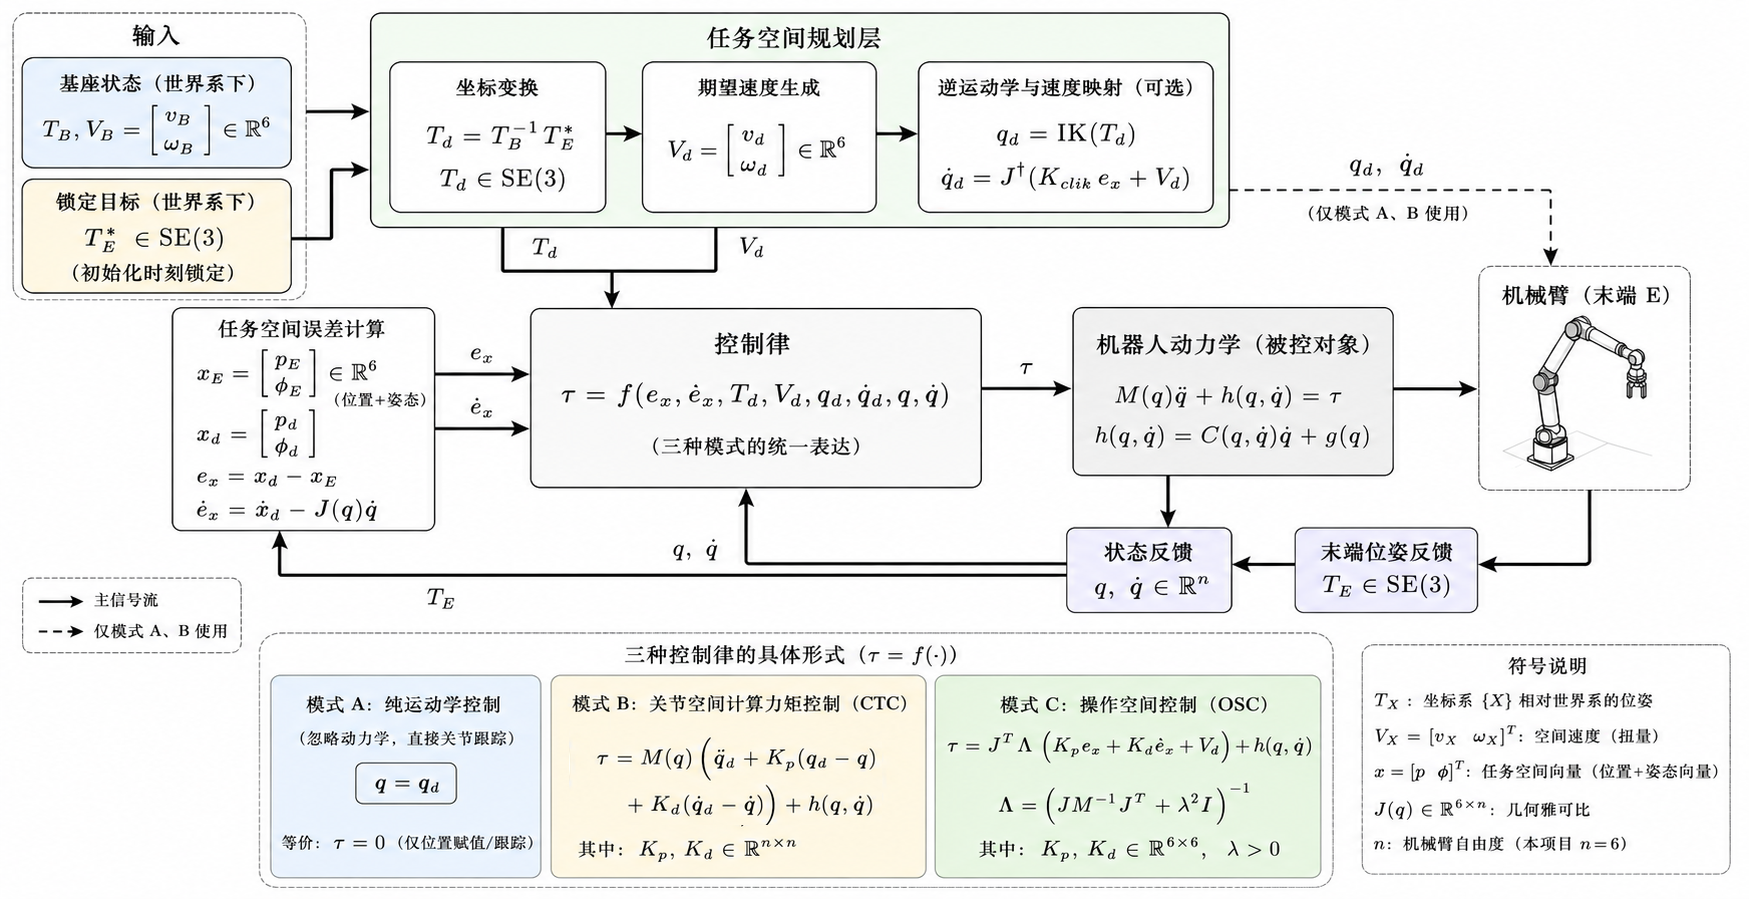
\includegraphics[width=1.05\linewidth]{1.png}
    \caption{三层架构：任务空间规划 $\rightarrow$ 控制律 $\rightarrow$ 执行层闭环。}
    \label{fig:arch}
\end{figure}

\begin{enumerate}[leftmargin=2em]
    \item 规划层：读取基座 $T_B$ 与锁定目标 $T_E^*$，计算基座系期望 $T_D$ 与补偿速度 $V_D$；再通过 IK/CLIK 得到关节参考 $q_D,\dot{q}_D$。
    \item 控制层：在 Kinematic / CTC / OSC 三种模式间择一，输出关节目标 $q_D$（模式 A）或关节力矩 $\tau$（模式 B/C）。
    \item 执行层：仿真中对 $\tau$ 做 ABA 动力学积分得到 $q,\dot{q}$；真机中将指令下发至 MIT 电机驱动。
\end{enumerate}

以模式 C 为例，单周期数据流为：
(1)~读取 $q,\dot{q}$ 与 $T_B$；
(2)~计算 $T_D,V_D$ 与 $e_x$；
(3)~OSC 算出 $\tau_{\mathrm{OSC}}$；
(4)~执行层积分/下发，更新 $T_E$；
(5)~下一周期重复。模式 A/B 在第 (3) 步分别替换为“$q\leftarrow q_D$”与 CTC 力矩计算。

\subsection{数据流}

\begin{table}[H]
  \centering
  \caption{系统级数据流（不含具体通信接口）}
  \label{tab:dataflow}
  \begin{tabular}{@{} l l l @{}}
    \toprule
    方向 & 信号 & 说明 \\
    \midrule
    输入 & $T_B$，$\dot{T}_B$ & 仿真 mount 或外部位姿估计 \\
    规划输出 & $T_D$，$V_D$，$q_D$，$\dot{q}_D$ & 三种模式共享 \\
    控制输出 & $q_D$ 或 $\tau$ & 依模式而定 \\
    反馈 & $q$，$\dot{q}$，$T_E$ & 关节状态与末端位姿 \\
    \bottomrule
  \end{tabular}
\end{table}

具体 ROS 2 话题映射见附录~\ref{app:ros}。

\subsection{三种执行模式概览}

\begin{table}[H]
  \centering
  \caption{三种执行模式概览}
  \label{tab:mode-overview}
  \begin{tabular}{@{} l l l @{}}
    \toprule
    模式 & 名称 & 控制空间 $\rightarrow$ 输出 \\
    \midrule
    A & Kinematic Control & 关节 $\rightarrow$ $q_D$ \\
    B & CTC & 关节 $\rightarrow$ $\tau_{\mathrm{CTC}}$ \\
    C & OSC & 任务 $\rightarrow$ $\tau_{\mathrm{OSC}}$ \\
    \bottomrule
  \end{tabular}
\end{table}

\subsection{设计思路}
\label{sec:design-rationale}

本节阐述系统架构的设计思路。整体遵循同一原则：在可对比、可分层的前提下，将末端稳定问题分解为规划、控制与执行三个可独立评估的环节；三模式、统一规划层与 Benchmark 路径均围绕这一原则展开。

\subsubsection{统一规划层}

规划层统一生成 $T_D$、$V_D$ 及（经 IK/CLIK 得到的）$q_D,\dot{q}_D$。上述量表达``在世界系中保持末端''的任务要求，与后续采用 Kinematic Control、CTC 或 OSC 无关。A/B/C 三种模式共用同一规划层输出，控制层仅替换第 3 步的映射关系（$q\leftarrow q_D$ / CTC / OSC）。

统一规划层保证以下三点：
\begin{enumerate}[label=(\arabic*), leftmargin=2.5em]
    \item 实验输入一致。三模式对比时，$T_B$、$T_E^*$、扰动工况与 $T_D,V_D$ 完全相同；性能差异仅来自控制律与执行链，而非规划侧参数漂移或实现分叉。
    \item 误差来源可分离。末端总误差可分解为
    \begin{equation}
        e_{\mathrm{total}}
        \;\approx\;
        e_{\mathrm{plan}} + e_{\mathrm{ctrl}} + e_{\mathrm{exec}},
        \label{eq:error-decomp}
    \end{equation}
    其中 $e_{\mathrm{plan}}$ 来自 $T_B\rightarrow T_D$ 变换、$V_D$ 生成与 IK/CLIK；$e_{\mathrm{ctrl}}$ 来自 CTC/OSC 闭环；$e_{\mathrm{exec}}$ 来自动力学积分、力矩限幅或电机跟踪。若各模式独立实现规划，则 $e_{\mathrm{plan}}$ 随模式变化，式~\eqref{eq:error-decomp} 无法成立，故障无法定位至具体层级。
    \item Benchmark 可比。模式 A 在统一输入下给出 $e_{\mathrm{plan}}$ 的定量上界（见~\S\ref{sec:mode-a-rationale}）；B/C 相对 A 的增量即 $e_{\mathrm{ctrl}}+e_{\mathrm{exec}}$，可在同一扰动工况下直接相减对比。
\end{enumerate}

本设计不采用``每模式独立规划''：除重复实现坐标变换与 $V_D$ 生成外，更根本的问题在于丧失分层诊断能力——无法判断``末端偏差大''究竟源于 $T_D$ 算错、IK 不收敛，还是 CTC/OSC 带宽不足。规划层因此固化为三种模式的唯一输入源，各模式独立规划不在设计范围内。

\subsubsection{三种控制模式}

系统提供 Kinematic Control、CTC、OSC 三种可切换控制模式，按能力递进组织：
\begin{center}
几何标定（A）$\;\longrightarrow\;$ 关节动力学补偿（B）$\;\longrightarrow\;$ 任务空间闭环（C）
\end{center}

三种模式构成能力阶梯，而非三个互不相关的备选方案：
\begin{itemize}[leftmargin=2em]
    \item 模式 A 忽略 $M,h$ 与力矩限幅，给出规划链路的几何性能上界；
    \item 模式 B 在 A 的基础上引入关节空间动力学闭环与低通，评估``关节力矩跟踪 $q_D$''的代价；
    \item 模式 C 跳过关节空间跟踪，在任务空间直接闭环，为真机部署主方案。
\end{itemize}

推荐工程流程：先用 A 标定规划层 $\rightarrow$ 用 B 评估关节动力学与力矩可行性 $\rightarrow$ 用 C 部署真机。模式切换用于回归测试；当末端性能异常时，按 A$\rightarrow$B$\rightarrow$C 顺序对比，逐层缩小故障范围（见表~\ref{tab:fault-isolation}）。

\begin{table}[H]
  \centering
  \caption{三模式对比时的故障分层逻辑}
  \label{tab:fault-isolation}
  \renewcommand{\arraystretch}{1.2}
  \begin{tabular}{@{} p{3.5cm} p{9.5cm} @{}}
    \toprule
    对比结果 & 指示 \\
    \midrule
    A 误差已大 & 问题在规划层：$T_D$/$V_D$ 变换、IK 或 mount 输入 \\
    A 小、B 大、C 小 & 问题在关节空间跟踪（CTC 带宽、低通滞后、$\ddot{q}_D$ 跟踪） \\
    A 小、C 大 & 问题在任务空间控制或执行层（OSC 增益、$\Lambda$ 奇异、力矩限幅） \\
    A $\approx$ C，均小 & 规划与控制均达标；动力学补偿有效 \\
    \bottomrule
  \end{tabular}
\end{table}

\subsubsection{保留 Kinematic Control 模式}
\label{sec:mode-a-rationale}

真机部署主方案为 OSC（模式 C）。模式 A 与 C 能力差异大，但本设计仍保留 A，因其承担不可替代的基准与诊断职能。

模式 A 在仿真中令 $q=q_D$、$\dot{q}=0$，不积分式~\eqref{eq:dynamics}，等价于假设``关节能瞬时到达 IK 输出''。因此 A 的末端误差 $e_{\mathrm{A}}$ 仅含 $e_{\mathrm{plan}}$，是几何性能上界：任何考虑动力学、力矩限幅或电机滞后的方案，其任务空间 RMS 不应系统性优于 A。

在统一规划层与相同扰动工况下，比较位置 RMS $e_{\mathrm{A}}$ 与 $e_{\mathrm{C}}$：
\begin{itemize}[leftmargin=2em]
    \item 若 $e_{\mathrm{C}} \approx e_{\mathrm{A}}$（本项目中 A 为 0.283\,mm，C 为 0.363\,mm，同量级）：说明 OSC 引入的动力学与执行代价很小，瓶颈不在控制层；
    \item 若 $e_{\mathrm{C}} \gg e_{\mathrm{A}}$（C 显著劣于 A）：说明 $e_{\mathrm{ctrl}}+e_{\mathrm{exec}}$ 占主导，问题在控制器或执行层（增益整定、力矩饱和、模型误差等），而非规划；
    \item 若 $e_{\mathrm{A}}$ 本身已大：应先排查 $T_D$、$V_D$、IK 与 mount 输入，再调 CTC/OSC——在规划未标定前整定控制增益无法收敛。
\end{itemize}

该对比逻辑是本项目三模式并存的核心理由：A 不是``简化版部署方案''，而是可量化的规划层 Benchmark。没有 A，则 C 的 0.363\,mm 无法判断``已经很好''还是``相对几何上界损失过大''。

除 Benchmark 外，A 还用于：（1）IK 与 $T_B\rightarrow T_D$ 坐标变换标定；（2）$T_D,V_D,q_D$ 参考轨迹的可视化检查；（3）新扰动工况或参数变更后的规划层回归；（4）与 B/C 联合的故障分层（表~\ref{tab:fault-isolation}）。

\subsubsection{解析期望速度}

本系统采用 mount 解析速度生成 $V_D$（~\S3.5），以避免仿真 500\,Hz 与真机 100\,Hz 在不同控制频率下对 $T_D$ 数值差分带来的相位延迟与噪声；差分方案还依赖跨周期的 $\Delta t$ 与历史缓存，真机 $T_B$ 来自 TF 时存在时间戳对齐问题。解析 $V_D$ 仅使用当前 mount 速度与 $T_B$，两侧同式，有利于规划层在仿真与真机间保持一致。

\subsubsection{模式 B 低通与模式 C 主方案}

IK 在冗余自由度上存在多解，帧间 $q_D$ 可能跳变；CTC 对 $\ddot{q}_D$ 敏感，直接使用 IK 输出会引起 $\tau$ 尖峰。模式 B 对 IK 输出的 $q_D$ 施加一阶低通（$\alpha=0.55$）以平滑参考，代价是相位滞后——B 的定位是``评估关节空间力矩跟踪的上限与代价''，而非真机主方案。

OSC 在任务空间直接最小化 $e_x$（式~\eqref{eq:ex}），控制目标与实验主评价指标 $\|p_E-p_E^*\|$、$\|e_R\|$ 一致；CTC 在关节空间跟踪 $q_D$，末端误差是 $q_D$ 跟踪误差的间接结果，二者不对等。真机采用 C，使控制优化目标与性能验收指标对齐。

\subsubsection{设计思路一览}
\begin{table}[H]
  \centering
  \caption{主要设计思路}
  \label{tab:design-decisions}
  \renewcommand{\arraystretch}{1.15}
  \begin{tabular}{@{} p{3.0cm} p{3.8cm} p{6.5cm} @{}}
    \toprule
    本设计思路 & 未采用方案 & 说明 \\
    \midrule
    世界系锁定 $T_E^*$ & 基座系常值目标 & 基座系常值目标随 $T_B$ 漂移，无法在世界系稳定 \\
    解析 $V_D$ & 对 $T_D$ 数值差分 & 仿真/真机频率差异下，差分易引入相位延迟与噪声 \\
    共享规划层 & 每模式独立规划 & 保证输入一致；使式~\eqref{eq:error-decomp} 可分离 \\
    保留模式 A & 仅保留 OSC & 几何上界 Benchmark；A$\approx$C / C$\gg$A 诊断控制品质 \\
    模式 B 低通 & IK 输出直送 CTC & 抑制 IK 跳变引起的 $\tau$ 尖峰；B 用于动力学评估 \\
    模式 C 主方案 & 仅关节空间 CTC & 控制目标与 $T_E$ 验收指标一致 \\
    \bottomrule
  \end{tabular}
\end{table}

%==============================================================================
\section{任务空间规划}
%==============================================================================

\subsection{坐标系定义}

$\{W\}$ 为惯性参考系；$\{B\}$ 固连 \texttt{base\_link}；$\{E\}$ 固连 \texttt{link6}。位姿 $T=(R,p)\in SE(3)$，$R\in SO(3)$，$p\in\mathbb{R}^3$。除 $T_D$ 在 $\{B\}$ 中表达外，其余位姿默认在 $\{W\}$ 中给出。

\subsection{世界系目标锁定}

启动时采样 $T_E(t_0)$，令 $T_E^*=T_E(t_0)$ 此后保持不变（式~\eqref{eq:lock-target}）。$T_D$ 由式~\eqref{eq:td} 在每个控制周期由 $T_B$ 与 $T_E^*$ 换算，将世界系锁定转化为基座系跟踪。

\subsection{基座系目标生成}

基座位姿由 mount 运动链给出（安装偏置 $z_{\mathrm{off}}=0.02$\,m）：
\begin{equation}
    T_{\mathrm{mount}} = T_{\mathrm{trans}}(p_m)\, R_x R_y R_z, \quad
    T_B = T_{\mathrm{mount}}\, T_z(z_{\mathrm{off}}).
\end{equation}
\begin{equation}
    T_D = T_B^{-1}\, T_E^*.
    \label{eq:td}
\end{equation}
记 $T_D=(R_D,p_D)$，$T_E=(R_E,p_E)$（均在 $\{B\}$ 系）。

\subsection{任务误差定义}

\begin{equation}
    e_p = p_D - p_E, \quad
    e_R = \Log\!\bigl(R_E^\top R_D\bigr), \quad
    e_x = \begin{bmatrix} e_p \\ e_R \end{bmatrix} \in \mathbb{R}^6.
    \label{eq:ex}
\end{equation}
姿态误差采用 $\Log(SO(3))$ 轴角表示，便于任务空间 PD 线性化。模式 C 直接对 $e_x$ 闭环；模式 A/B 经 IK 映射为 $q_D$。

\subsection{期望速度生成}

本系统采用解析速度生成 $V_D$，以避免仿真（500\,Hz）与真机（100\,Hz）在不同控制频率下对 $T_D$ 数值差分带来的相位延迟与噪声（见附录~\ref{app:failure}）。

mount 角速度：$\omega = \dot{r}\mathbf{e}_x + R_x\dot{p}\mathbf{e}_y + R_xR_y\dot{y}\mathbf{e}_z$。平移分量：
\begin{equation}
    V_{D,\mathrm{trans}} = -R_B^\top\bigl(\dot{p}_m + \omega \times p_{\mathrm{off}} + \omega \times p_{\mathrm{rel}}\bigr),
    \label{eq:vd-trans}
\end{equation}
$p_{\mathrm{rel}}=p_E^*-p_B$。旋转分量由 $T_D$ 单步传播：
\begin{equation}
    V_{D,\mathrm{rot}} = \frac{\Log\!\bigl(R_D(t)^\top R_D(t+\Delta t)\bigr)}{\Delta t}.
    \label{eq:vd-rot}
\end{equation}
拼接 $V_D=[V_{D,\mathrm{trans}};V_{D,\mathrm{rot}}]$，各分量限幅 $[-15,15]$。

\subsection{逆运动学与速度前馈}

\subsubsection{逆运动学}

阻尼最小二乘（DLS）在速度层由任务误差解算关节角速度：
\begin{equation}
    \dot{q} = J(q)^\top \bigl(J(q)J(q)^\top + \lambda_{\mathrm{IK}}^2 I_6\bigr)^{-1} e_x,
    \quad \lambda_{\mathrm{IK}}=0.012.
    \label{eq:ik}
\end{equation}
式~\eqref{eq:ik} 给出使 $e_x$ 下降最快的关节运动方向。位置级 IK 对其做离散积分
$q \leftarrow q + \alpha\,\dot{q}$（步长缩放 $\alpha=0.9$，单关节单步限幅 0.2\,rad），迭代直至 $e_x$ 收敛，得 $q_D$；未收敛时依次增加 refine / recovery 迭代次数。

\subsubsection{关节速度前馈（CLIK）}

\begin{equation}
    \dot{q}_D = J(q)^\top \bigl(J(q)J(q)^\top + \lambda_{\mathrm{CLIK}}^2 I_6\bigr)^{-1}
    \bigl(K_x\, e_x + V_D\bigr),
    \label{eq:clik}
\end{equation}
$\lambda_{\mathrm{CLIK}}=0.05$，$K_x=\mathrm{diag}(8,8,8,6,6,6)$，$\dot{q}_D$ 限幅 3.0\,rad/s。

%==============================================================================
\section{控制方法}
\label{sec:control}

\subsection{控制思想}
\label{sec:control-philosophy}

三种模式共用规划层输出 $T_D,V_D$，差异在于闭环所在空间与所最小化的误差量。本节给出各模式的控制思想（Control Philosophy）；后续各小节给出具体控制律。

\begin{table}[H]
  \centering
  \caption{三模式控制思想对照}
  \label{tab:control-philosophy}
  \renewcommand{\arraystretch}{1.25}
  \begin{tabular}{@{} l l l l @{}}
    \toprule
    模式 & 控制思想 & 控制目标 & 闭环变量 \\
    \midrule
    A & 几何极限 & $T_E \rightarrow T_D$（无动力学） & $q = q_D$ \\
    B & Joint-space tracking & $q \rightarrow q_D$ & $\|q - q_D\|$ \\
    C & Task-space regulation & $T_E \rightarrow T_D$ & $\|e_x\|$ \\
    \bottomrule
  \end{tabular}
\end{table}

\paragraph{模式 A：几何极限（Geometric Limit）。}
模式 A 假设关节能瞬时到达 IK 输出，不积分动力学式~\eqref{eq:dynamics}。其末端误差仅反映规划层（$T_D,V_D$、IK）的几何精度，是 $e_{\mathrm{plan}}$ 的定量上界（~\S\ref{sec:mode-a-rationale}）。模式 A 回答的问题不是``如何更好地控制''，而是``在理想几何条件下，规划链路最多能做多好''。

\paragraph{模式 B：关节空间跟踪（Joint-space Tracking）。}
CTC 在关节空间闭环，控制目标是使实际关节状态跟踪规划给出的参考：
\begin{equation}
    q \rightarrow q_D, \qquad \dot{q} \rightarrow \dot{q}_D.
    \label{eq:ctrl-obj-b}
\end{equation}
式~\eqref{eq:ctc} 中的 $K_P(q_D-q)+K_D(\dot{q}_D-\dot{q})$ 直接惩罚关节跟踪误差；力矩 $\tau_{\mathrm{CTC}}$ 服务于式~\eqref{eq:ctrl-obj-b}，而非直接作用于 $e_x$。末端位姿 $T_E$ 由正运动学间接决定：即使 $\|q-q_D\|$ 较小，$T_E$ 仍可能偏离 $T_D$——冗余自由度 IK 多解、奇异位形与非线性映射均会在关节→末端路径上引入额外误差。因此，B 的主评价指标虽仍用任务空间 RMS（$\|p_E-p_E^*\|$、$\|e_R\|$），但控制优化目标与验收指标不一致；末端性能是关节跟踪质量的间接结果。

\paragraph{模式 C：任务空间调节（Task-space Regulation）。}
OSC 在任务空间闭环，控制目标是使实际末端位姿跟踪规划期望：
\begin{equation}
    T_E \rightarrow T_D
    \quad \Longleftrightarrow \quad
    e_x \rightarrow 0.
    \label{eq:ctrl-obj-c}
\end{equation}
式~\eqref{eq:osc} 中的 $K_P e_x + K_D \dot{e}_x$ 直接在任务空间施加 PD 反馈；$\tau_{\mathrm{OSC}}$ 服务于式~\eqref{eq:ctrl-obj-c}。$q_D$ 由 IK 并行计算，不进入控制律。

实验主评价为任务空间误差 $\|p_E-p_E^*\|$ 与 $\|e_R\|$（表~\ref{tab:metrics}），二者均由 $e_x$ 导出。对模式 C，控制目标式~\eqref{eq:ctrl-obj-c} 与验收指标一致：控制器所最小化的量即为实验所测量的量。这是 OSC 相对 CTC 的核心优势来源——CTC 优化 $\|q-q_D\|$，却在任务空间接受验收；二者之间经 $J(q)$ 与非线性正运动学耦合，无保证 $\|q-q_D\|$ 小则 $\|e_x\|$ 小。本项目中 B 位置 RMS 2.808\,mm、C 为 0.363\,mm 的差距，即这一控制思想差异的直接体现。

三种模式按能力递进组织：A 给出几何极限 $\rightarrow$ B 评估关节力矩跟踪的代价 $\rightarrow$ C 在任务空间直接调节并作为真机主方案。

\subsection{模式 A：Kinematic Control}

模式 A 忽略关节动力学，直接将关节角设为 IK 输出：
\begin{equation}
    q = q_D, \quad \dot{q} = 0, \quad \tau = 0.
\end{equation}
仿真中不积分式~\eqref{eq:dynamics}，直接令 $q=q_D$、$\dot{q}=0$；真机由 MIT 位置环跟踪 $q_D$，力矩前馈为零。承担规划层 Benchmark（~\S\ref{sec:mode-a-rationale}），不作为真机部署方案。

\subsection{模式 B：CTC}

CTC 实现关节空间跟踪（式~\eqref{eq:ctrl-obj-b}）。IK 输出的 $q_D$ 帧间可能因冗余解跳变；对其施加一阶低通（$\alpha=0.55$）后再作为 CTC 参考，在平滑性与相位滞后之间折中。

\subsubsection{控制律}

对低通后的 $q_D$，计算关节力矩：
\begin{equation}
    \tau = \tau_{\mathrm{CTC}}
    = M(q)\left(
    \ddot{q}_D + K_P(q_D - q) + K_D(\dot{q}_D - \dot{q})
    \right) + h(q,\dot{q}),
    \label{eq:ctc}
\end{equation}
式~\eqref{eq:ctc} 为“逆动力学 + PD 反馈”的标准形式，逐项含义：
\begin{itemize}[leftmargin=2em]
    \item $\ddot{q}_D$：期望关节加速度（由 $\dot{q}_D$ 差分或规划给出），前馈轨迹；
    \item $K_P(q_D-q)+K_D(\dot{q}_D-\dot{q})$：关节位置/速度 PD 反馈，缩小跟踪误差；
    \item $M(q)[\cdots]$：将期望加速度与反馈加速度映射为所需力矩；
    \item $+h(q,\dot{q})$：补偿重力与科氏/离心项，使 $\ddot{q}$ 更接近指令值。
\end{itemize}
增益 $K_P,K_D$ 为 $6\times 6$ 对角矩阵（见附录~\ref{app:params}）。信号链路：
$T_D,V_D \rightarrow \mathrm{IK} \rightarrow \mathrm{LPF}(q_D) \rightarrow \mathrm{CTC} \rightarrow \mathrm{ABA} \rightarrow T_E$。

\subsection{模式 C：OSC}

OSC 实现任务空间调节（式~\eqref{eq:ctrl-obj-c}）。信号链路：
$T_D,V_D \rightarrow e_x \rightarrow \tau_{\mathrm{OSC}} \rightarrow T_E$。
$q_D$ 仅作遥测。真机部署采用本模式。

\subsubsection{控制律}

先计算操作空间惯量 $\Lambda$，它描述“在末端施加单位加速度需要多少关节力矩”：
\begin{equation}
    \Lambda = \bigl(J(q)\, M(q)^{-1}\, J(q)^\top + \lambda_{\mathrm{OSC}}^2 I_6\bigr)^{-1},
    \label{eq:lambda}
\end{equation}
$\lambda_{\mathrm{OSC}}^2 I_6$ 为阻尼正则化，避免 $J$ 奇异时 $\Lambda$ 过大。任务误差变化率为
\begin{equation}
    \dot{e}_x = V_D - J(q)\,\dot{q},
\end{equation}
即“期望末端速度减实际末端速度”。最终力矩为
\begin{equation}
    \tau = \tau_{\mathrm{OSC}}
    = J(q)^\top \Lambda \bigl(K_P e_x + K_D \dot{e}_x\bigr) + h(q,\dot{q}),
    \label{eq:osc}
\end{equation}
式~\eqref{eq:osc} 的含义：$K_P e_x + K_D \dot{e}_x$ 为任务空间 PD 指令（期望末端加速度）；$\Lambda$ 将其转为等效力矩；$J^\top$ 映射回关节；$+h$ 补偿非线性项。任务空间增益 $K_P,K_D$ 分平移/旋转通道整定；任务加速度限幅 $\pm 220$ 后映射为 $\tau_{\mathrm{OSC}}$，防止力矩过大。

\subsection{三模式对比}

\begin{table}[H]
  \centering
  \caption{三种控制方法对比}
  \label{tab:mode-compare}
  \begin{tabular}{@{} l l l l l @{}}
    \toprule
    模式 & 控制思想 & 控制目标 & 关节参考 $q_D$ & 输出 \\
    \midrule
    A & 几何极限 & $T_E\!\rightarrow\! T_D$（无动力学） & IK 直接 & $q=q_D$ \\
    B & Joint-space tracking & $q\!\rightarrow\! q_D$ & 低通 $q_D$ & $\tau_{\mathrm{CTC}}$ \\
    C & Task-space regulation & $T_E\!\rightarrow\! T_D$ & 仅遥测 & $\tau_{\mathrm{OSC}}$ \\
    \bottomrule
  \end{tabular}
\end{table}

%==============================================================================
\section{执行层实现}
%==============================================================================

\subsection{控制频率}

\begin{table}[H]
  \centering
  \caption{控制频率配置}
  \label{tab:freq}
  \begin{tabular}{@{} l l l @{}}
    \toprule
    层级 & 频率 & 配置说明 \\
    \midrule
    仿真规划+控制 & 500\,Hz & 与 ABA 积分步长匹配，减小离散化误差 \\
    真机规划+控制 & 100\,Hz & 匹配 \texttt{student\_arm\_node} 10\,ms 周期与电机总线带宽 \\
    真机 MIT 执行 & 100\,Hz & 与上层指令同频，降低延迟失配 \\
    \bottomrule
  \end{tabular}
\end{table}

\subsection{仿真执行链}

模式 B/C：对 $\tau$ 逐分量限幅 $|\tau_i|\le 85$\,Nm 后，用 ABA 算法积分式~\eqref{eq:dynamics}：
\begin{equation}
    \ddot{q}=M(q)^{-1}\bigl(\tau-h(q,\dot{q})\bigr),
\end{equation}
得到新的 $\dot{q},q$（再经关节限幅）。模式 A 跳过积分，直接令 $q=q_D$、$\dot{q}=0$。每步将关节状态发布至 \texttt{/joint\_states}，并由正运动学计算 $T_E$。

\subsection{真机执行链}

上层 \texttt{ee\_stabilization} 节点输出 $(q_D,\dot{q}_D,\tau)$；下层 \texttt{student\_arm\_node} 采用 MIT 阻抗模式，将 $\tau$ 作为力矩前馈，由电机内环完成位置跟踪：
\begin{equation}
    \tau_{\mathrm{motor}} = K_P(q_D - q) + K_D(\dot{q}_D - \dot{q}) + \tau.
    \label{eq:mit}
\end{equation}
式~\eqref{eq:mit} 中三项分别为：位置误差产生的阻抗力矩、速度误差产生的阻尼力矩、上层控制律给出的前馈力矩。此处 $K_P,K_D$ 为电机层阻抗增益，与式~\eqref{eq:ctc}、\eqref{eq:osc} 中的 CTC/OSC 增益不是同一组参数——前者决定电机如何跟踪 $q_D$，后者决定上层如何计算 $\tau$。电机层数值及 \texttt{yaml} 字段名见附录~\ref{app:params}。

\subsection{安全机制}

\begin{table}[H]
  \centering
  \caption{安全机制一览}
  \label{tab:safety}
  \renewcommand{\arraystretch}{1.2}
  \begin{tabular}{@{} p{2.8cm} p{4.5cm} p{6.5cm} @{}}
    \toprule
    类别 & 机制 & 实现位置 \\
    \midrule
    力矩保护 & 仿真 $|\tau|\le 85$\,Nm；真机 $|\tau|\le 9$\,Nm & 控制节点 \\
    任务加速度限幅 & OSC $\|a_{\mathrm{task}}\|_\infty\le 220$ & 动力学模块 \\
    限位保护 & $q_D$ 钳制至关节上下限 & 执行节点 \\
    超时保护 & 0.5\,s 无新指令则保持当前 $q$ & 执行节点 \\
    NaN/Inf 拒绝 & 非法指令不写入电机 & 执行节点 \\
    初始姿态 & 启动配置 $q_{\mathrm{home}}$ & 参数文件 \\
    奇异位形 & DLS 阻尼 $\lambda_{\mathrm{IK}},\lambda_{\mathrm{CLIK}}$ & 规划层 \\
    \bottomrule
  \end{tabular}
\end{table}

注：当前未实现独立硬件急停链路；安全依赖力矩限幅、限位与超时保持。外场部署须叠加飞控级急停。

%==============================================================================
\section{实验平台}
%==============================================================================

\begin{table}[H]
  \centering
  \caption{实验平台配置}
  \label{tab:platform}
  \begin{tabular}{@{} l l @{}}
    \toprule
    项目 & 配置 \\
    \midrule
    机械臂 & A-L1-GAMMA，6 自由度 + 1 固定关节 \\
    动力学模型 & Pinocchio（\texttt{single\_arm.urdf}） \\
    仿真环境 & ROS 2 Humble，headless launch，无 RViz \\
    控制节点 & \texttt{ee\_stabilization}，单进程规划+控制 \\
    计算平台 & 标准 x86\_64 Linux（WSL2 兼容） \\
  \bottomrule
  \end{tabular}
\end{table}

基座扰动在仿真中由内置 mount 模型提供（球内随机轨迹）；实验评价在完整闭环下进行。

%==============================================================================
\section{实验方法}
%==============================================================================

\subsection{扰动与工况}

基座在半径约 0.32\,m 球内做平滑随机平移与姿态扰动（段内时间常数 2.0\,s），模拟无人机晃动。启动后锁定 $T_E^*$，全程跟踪。

\subsection{自动测试流程}

脚本 \texttt{test\_all\_modes.py}：预热 2.5\,s $\rightarrow$ 记录 7\,s $\rightarrow$ 三模式依次运行。采样约 50\,Hz。

\subsection{评价指标}

实验从任务空间（末端位姿）与关节空间两个层面评价性能。任务空间指标在三模式间定义一致，可直接横向对比；关节类指标因控制目标不同而分模式定义（见表~\ref{tab:metrics}）。

\begin{table}[H]
  \centering
  \caption{评价指标定义（按模式）}
  \label{tab:metrics}
  \renewcommand{\arraystretch}{1.25}
  \small
  \begin{tabularx}{\textwidth}{@{} >{\raggedright\arraybackslash}p{2.4cm} X >{\raggedright\arraybackslash}p{2.6cm} @{}}
    \toprule
    指标 & 定义 & 适用模式 \\
    \midrule
    位置误差 & $\|p_E-p_E^*\|$（mm），末端位置与世界系目标之距离 & A/B/C \\
    姿态误差 & $\|e_R\|$（$^\circ$），姿态轴角偏差范数 & A/B/C \\
    关节参考误差 & $\|q-q_D\|$，$q_D$ 为 IK 输出 & 模式 A \\
    关节跟踪误差 & $\|q-q_D\|$，$q_D$ 为低通后 CTC 目标 & 模式 B \\
    IK 参考偏差 & $\|q-q_D\|$，$q_D$ 为并行 IK 遥测 & 模式 C（诊断） \\
    \bottomrule
  \end{tabularx}
\end{table}

表中 $p_E^*$ 为 $T_E^*$ 的位置部分；$e_R$ 由式~\eqref{eq:ex} 定义。$N$ 为采样点数，$\bar{e}$ 为均值，$e_{\max}$ 为峰值，RMS 为均方根——RMS 越大表示整体偏差越大。任务空间指标是三种模式的主评价；模式 C 的 $|q-q_D|$ 不参与性能排名，因 OSC 不跟踪 $q_D$。

\subsection{数据同步}

$q$ 与 $q_D$ 按消息时间戳配对，避免异步采样引入伪尖刺（详见附录~\ref{app:failure}）。

%==============================================================================
\section{实验结果}
%==============================================================================

\subsection{位置误差}

\begin{table}[H]
  \centering
  \caption{位置误差 $\|p_E - p_E^*\|$（mm）}
  \label{tab:exp-pos}
  \begin{tabular}{@{} l c c c c @{}}
    \toprule
    模式 & $N$ & $\bar{e}$ & $e_{\max}$ & RMS \\
    \midrule
    A & 270 & 0.245 & 0.499 & 0.283 \\
    B & 358 & 2.094 & 9.507 & 2.808 \\
    C & 359 & 0.325 & 0.687 & 0.363 \\
    \bottomrule
  \end{tabular}
\end{table}

\begin{figure}[H]
    \centering
    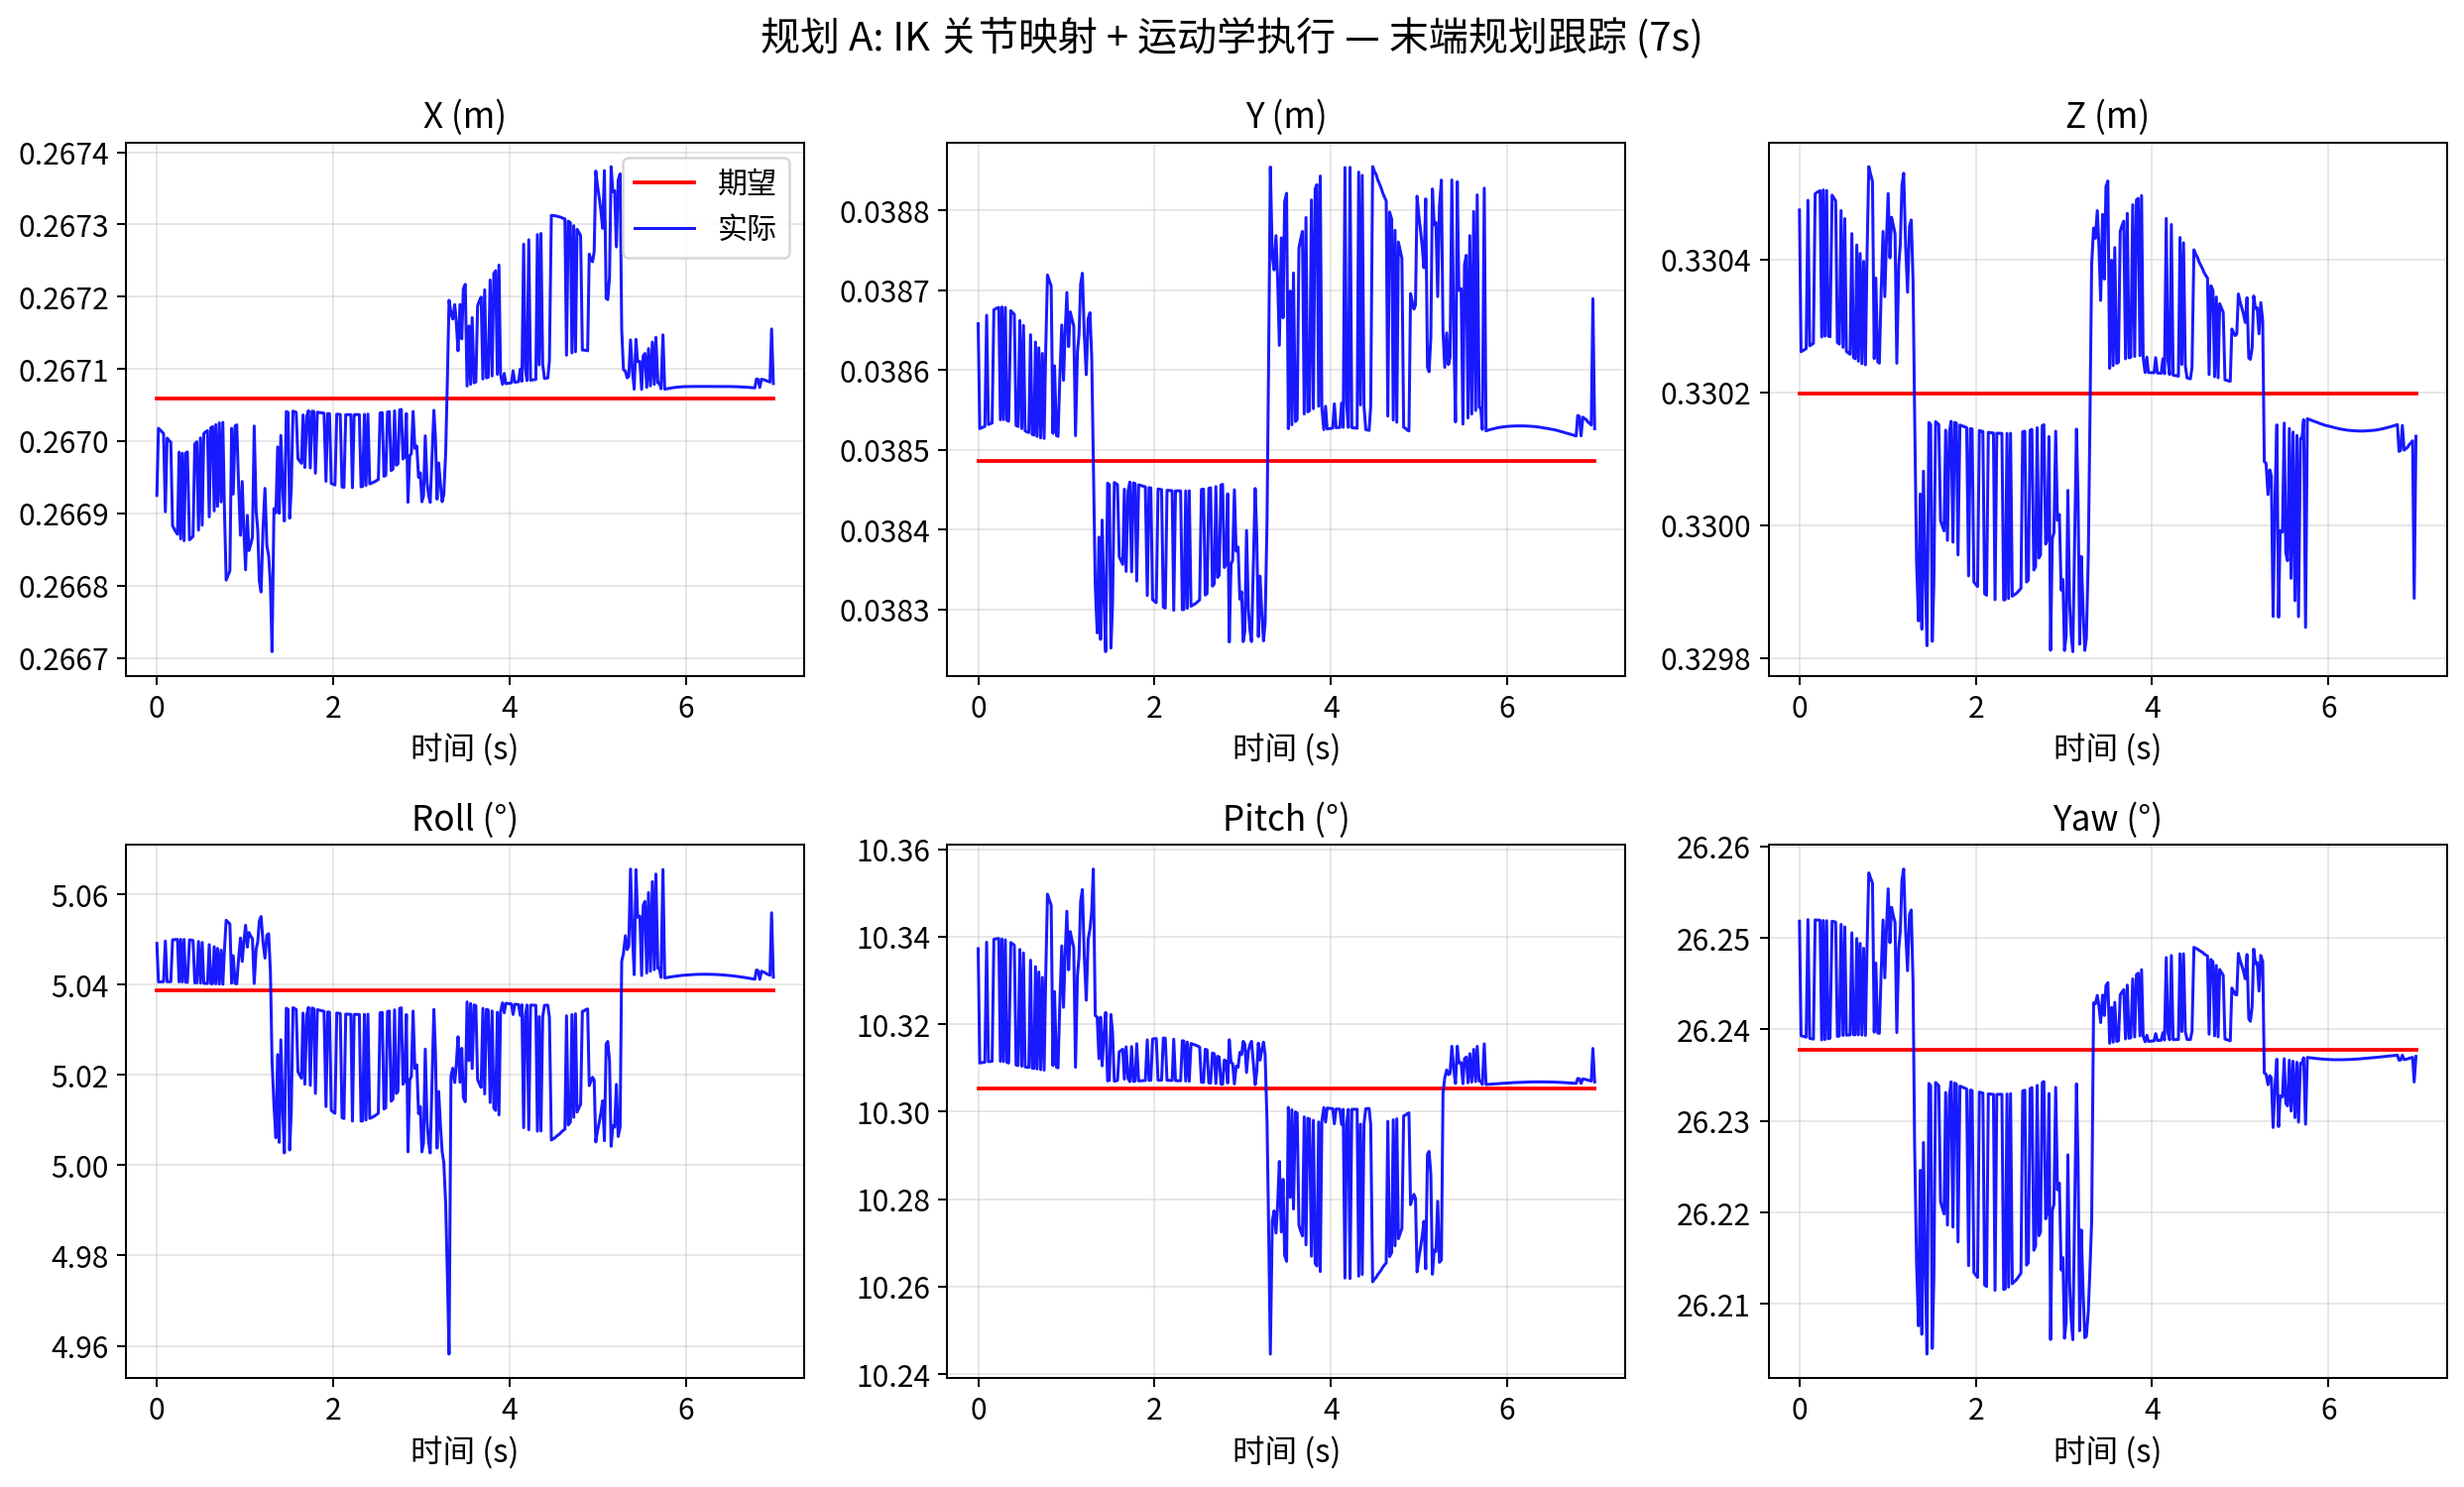
\includegraphics[width=0.92\linewidth]{mode_A_planning.png}
    \caption{模式 A：$p_E$ vs 目标}
\end{figure}
\begin{figure}[H]
    \centering
    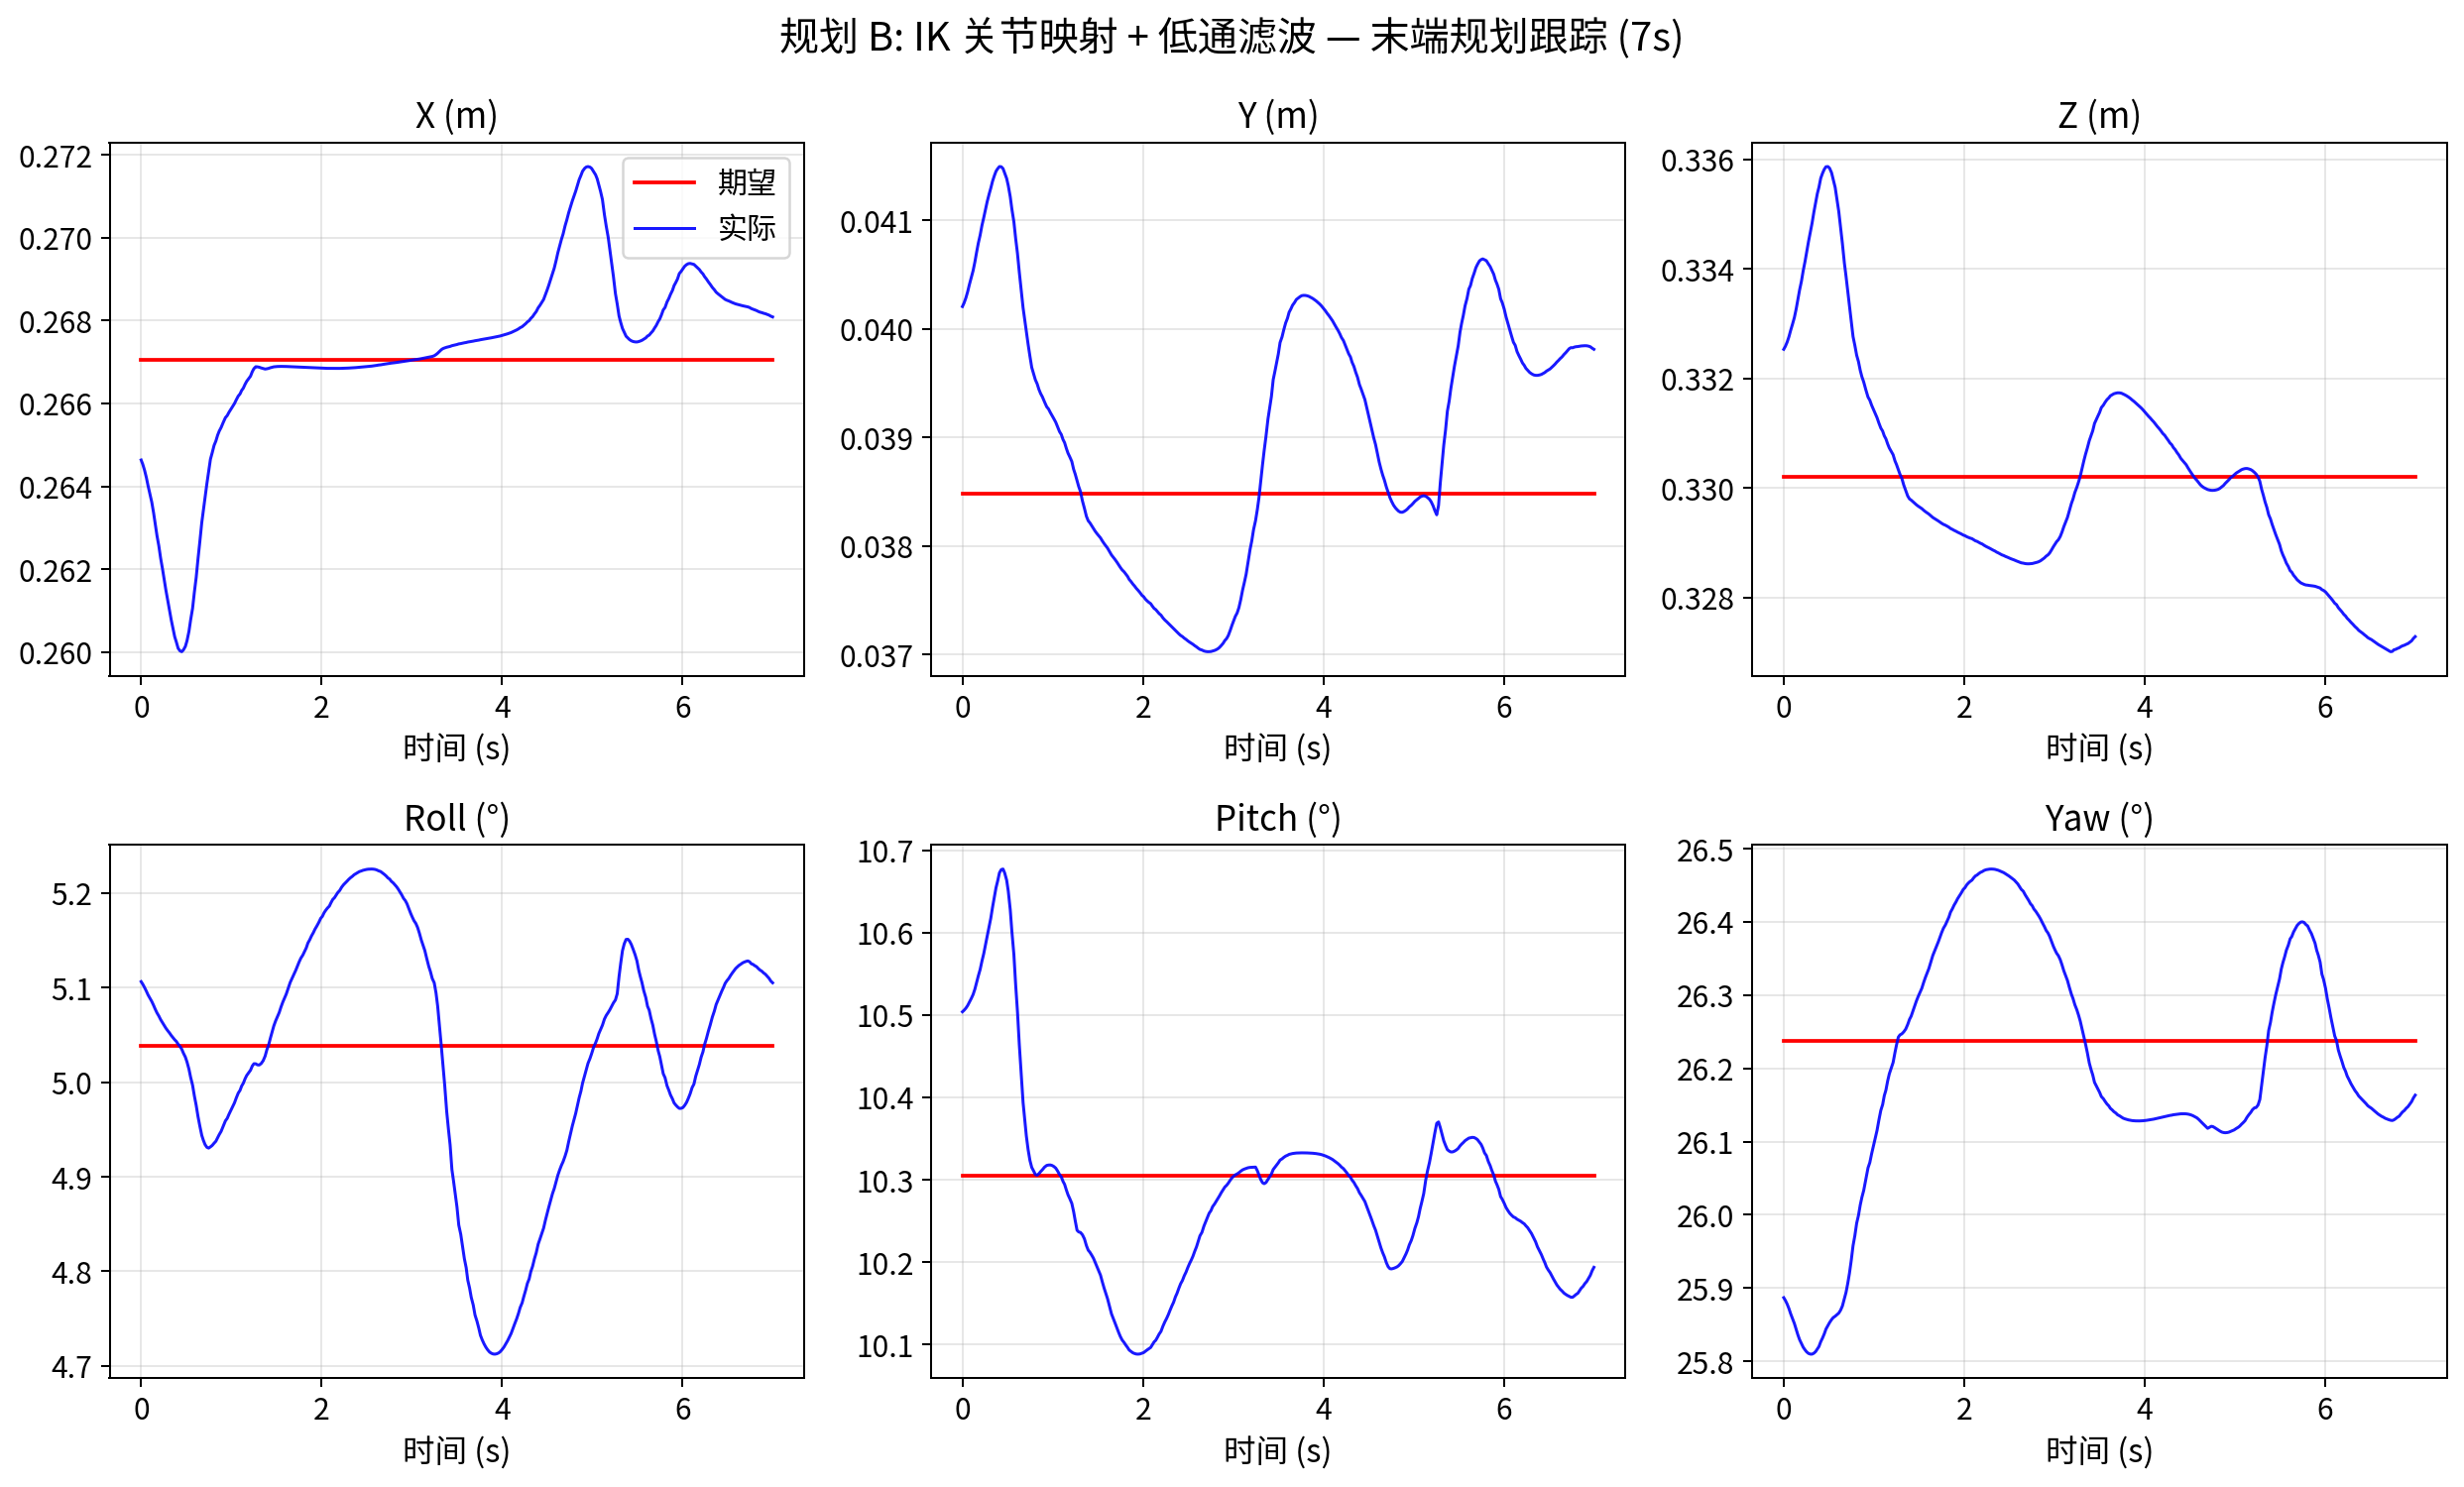
\includegraphics[width=0.92\linewidth]{mode_B_planning.png}
    \caption{模式 B：$p_E$ vs 目标}
    \label{fig:mode-B-planning}
\end{figure}
\begin{figure}[H]
    \centering
    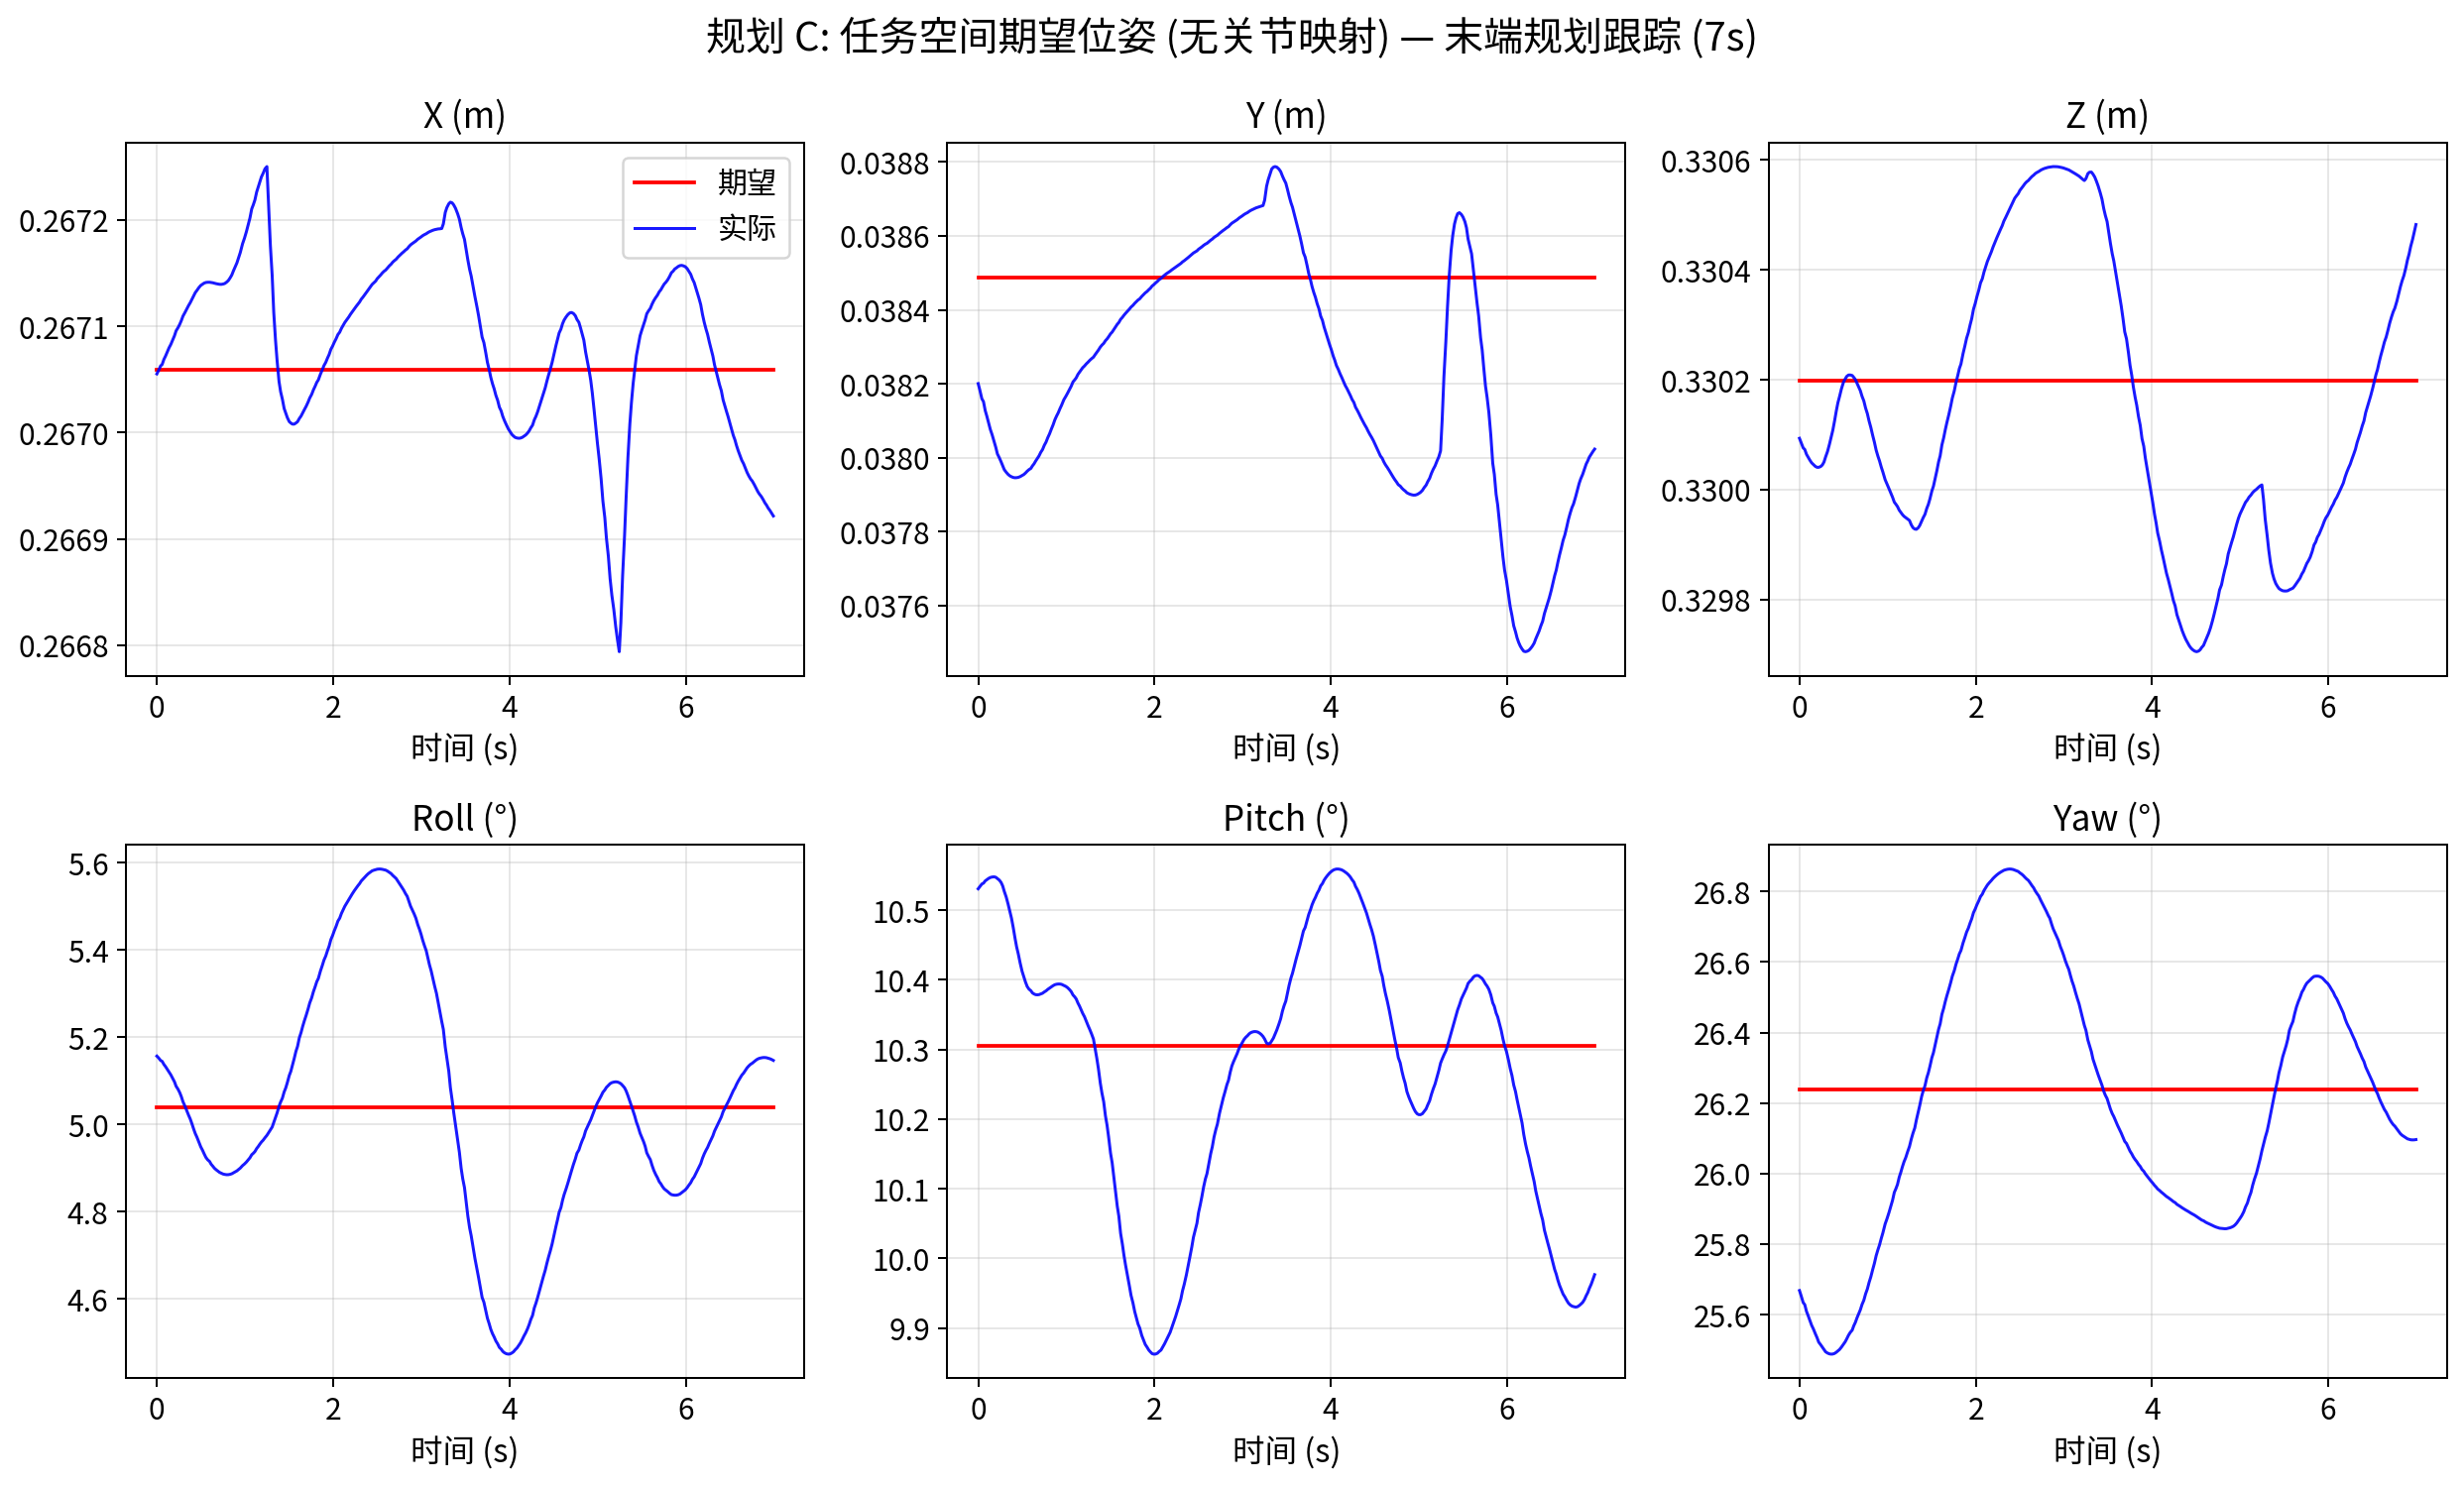
\includegraphics[width=0.92\linewidth]{mode_C_planning.png}
    \caption{模式 C：$p_E$ vs 目标}
\end{figure}

\subsection{姿态误差}

\begin{table}[H]
  \centering
  \caption{姿态误差 $\|e_R\|$（$^\circ$）}
  \label{tab:exp-ang}
  \begin{tabular}{@{} l c c c c @{}}
    \toprule
    模式 & $N$ & $\bar{e}$ & $e_{\max}$ & RMS \\
    \midrule
    A & 270 & 0.0308 & 0.0997 & 0.0371 \\
    B & 358 & 0.2264 & 0.5512 & 0.2582 \\
    C & 359 & 0.4431 & 0.8838 & 0.5066 \\
    \bottomrule
  \end{tabular}
\end{table}

\subsection{关节空间指标}

\begin{table}[H]
  \centering
  \caption{关节类指标（分模式定义，单位：rad）}
  \label{tab:exp-joint}
  \begin{tabular}{@{} l l c c c c @{}}
    \toprule
    模式 & 指标含义 & $N$ & $\bar{e}$ & $e_{\max}$ & RMS \\
    \midrule
    A & 关节参考误差 $\|q-q_D\|$ & 270 & 0.0000 & 0.0000 & 0.0000 \\
    B & 关节跟踪误差 $\|q-q_D\|$ & 358 & 0.0321 & 0.263 & 0.0610 \\
    C & IK 参考偏差 $\|q-q_D\|$（非控制目标） & 359 & 0.0088 & 0.050 & 0.0142 \\
    \bottomrule
  \end{tabular}
\end{table}

\begin{figure}[H]
    \centering
    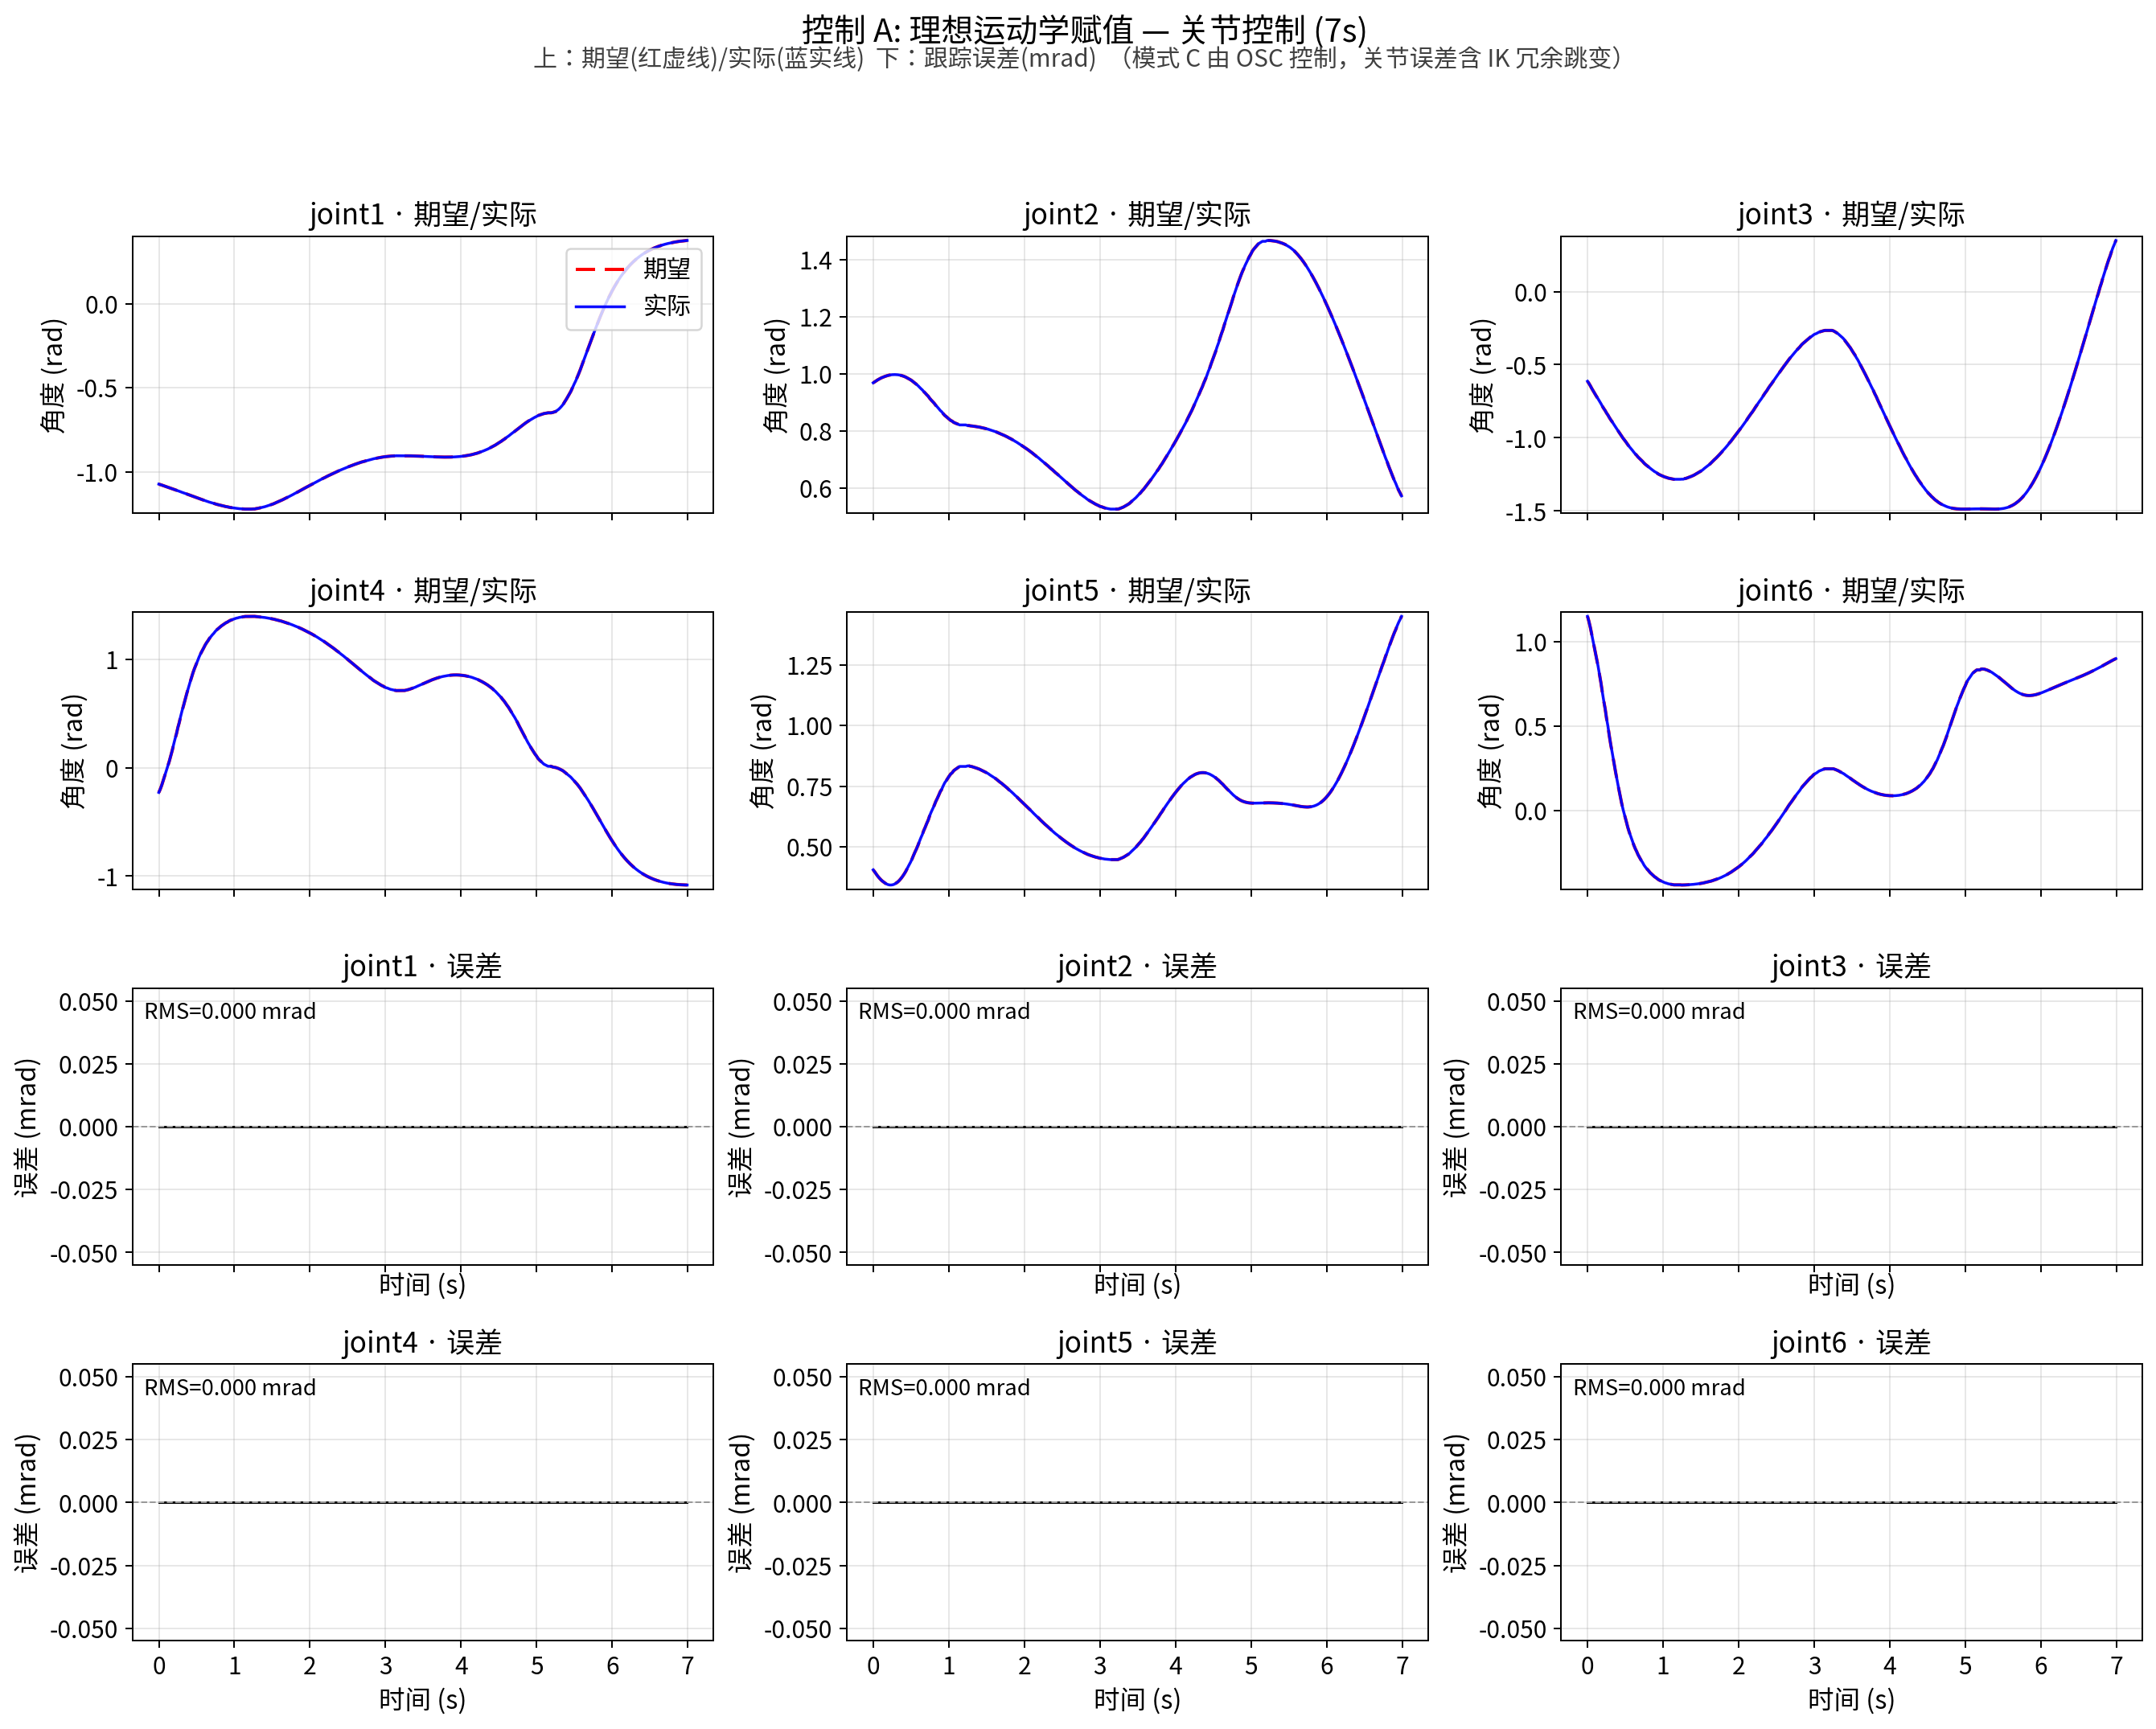
\includegraphics[width=0.92\linewidth]{mode_A_control.png}
    \caption{模式 A：关节参考误差 $|q-q_D|$}
\end{figure}
\begin{figure}[H]
    \centering
    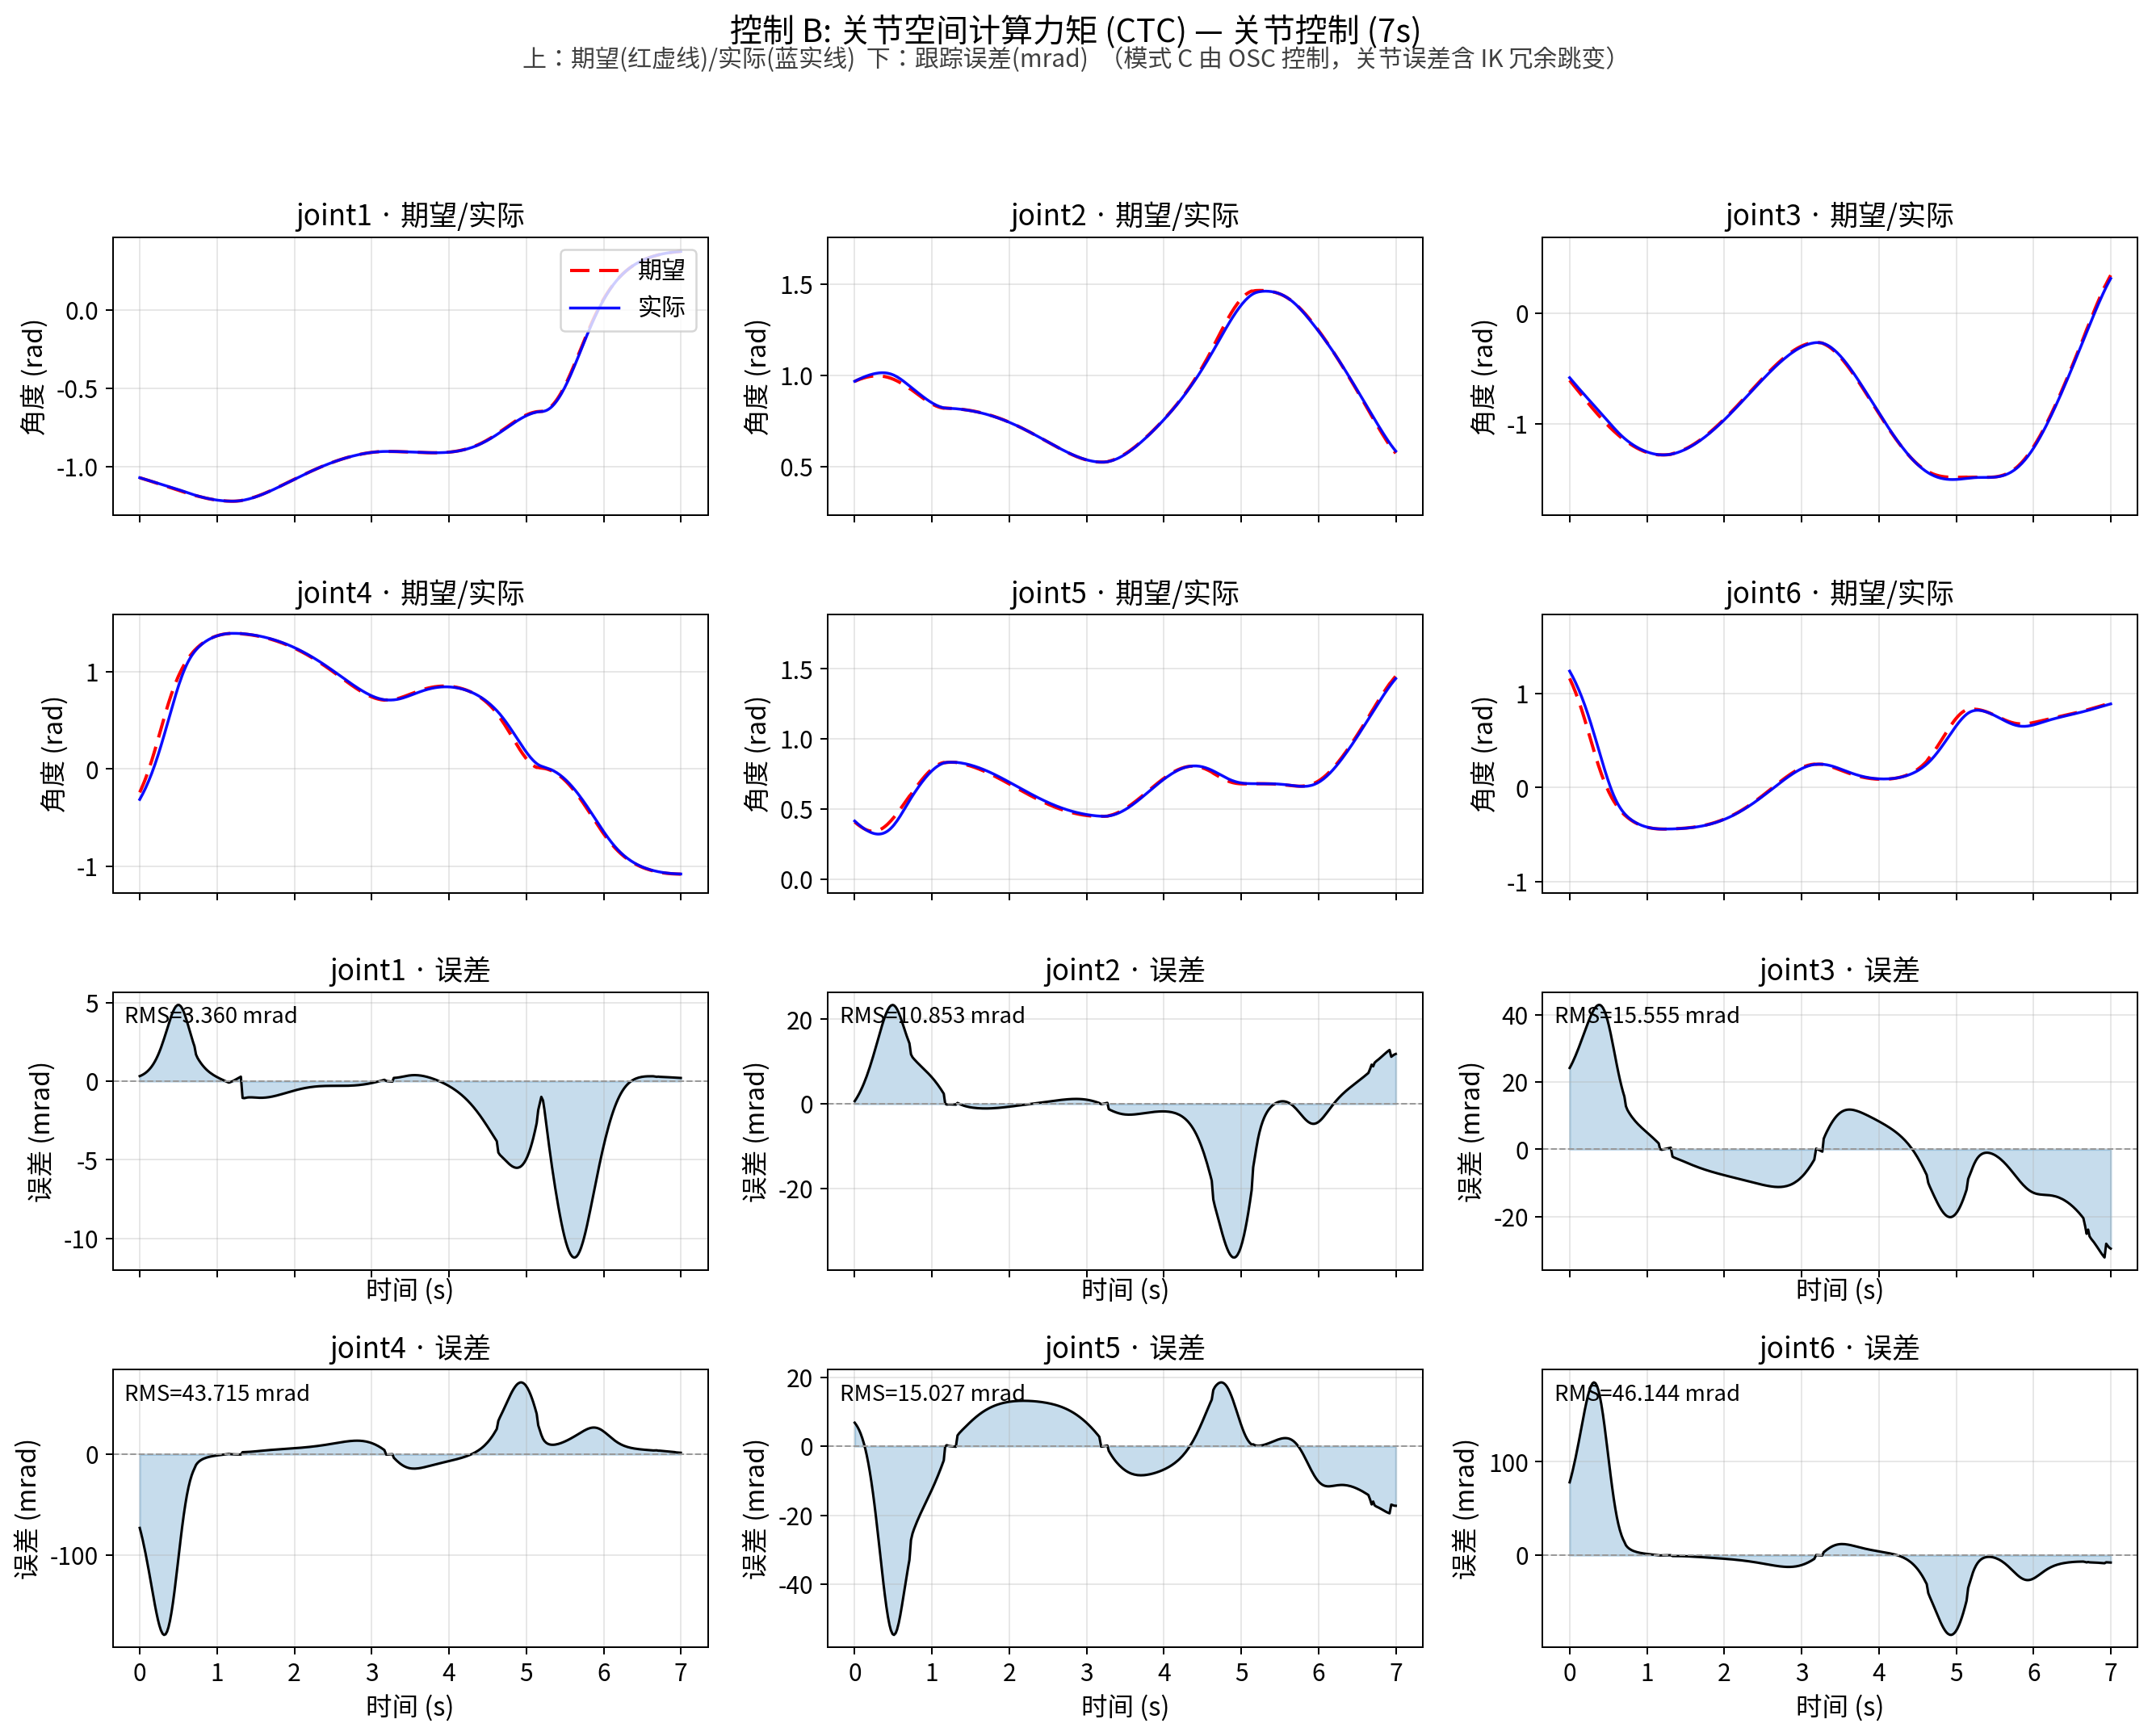
\includegraphics[width=0.92\linewidth]{mode_B_control.png}
    \caption{模式 B：关节跟踪误差 $|q-q_D|$}
\end{figure}
\begin{figure}[H]
    \centering
    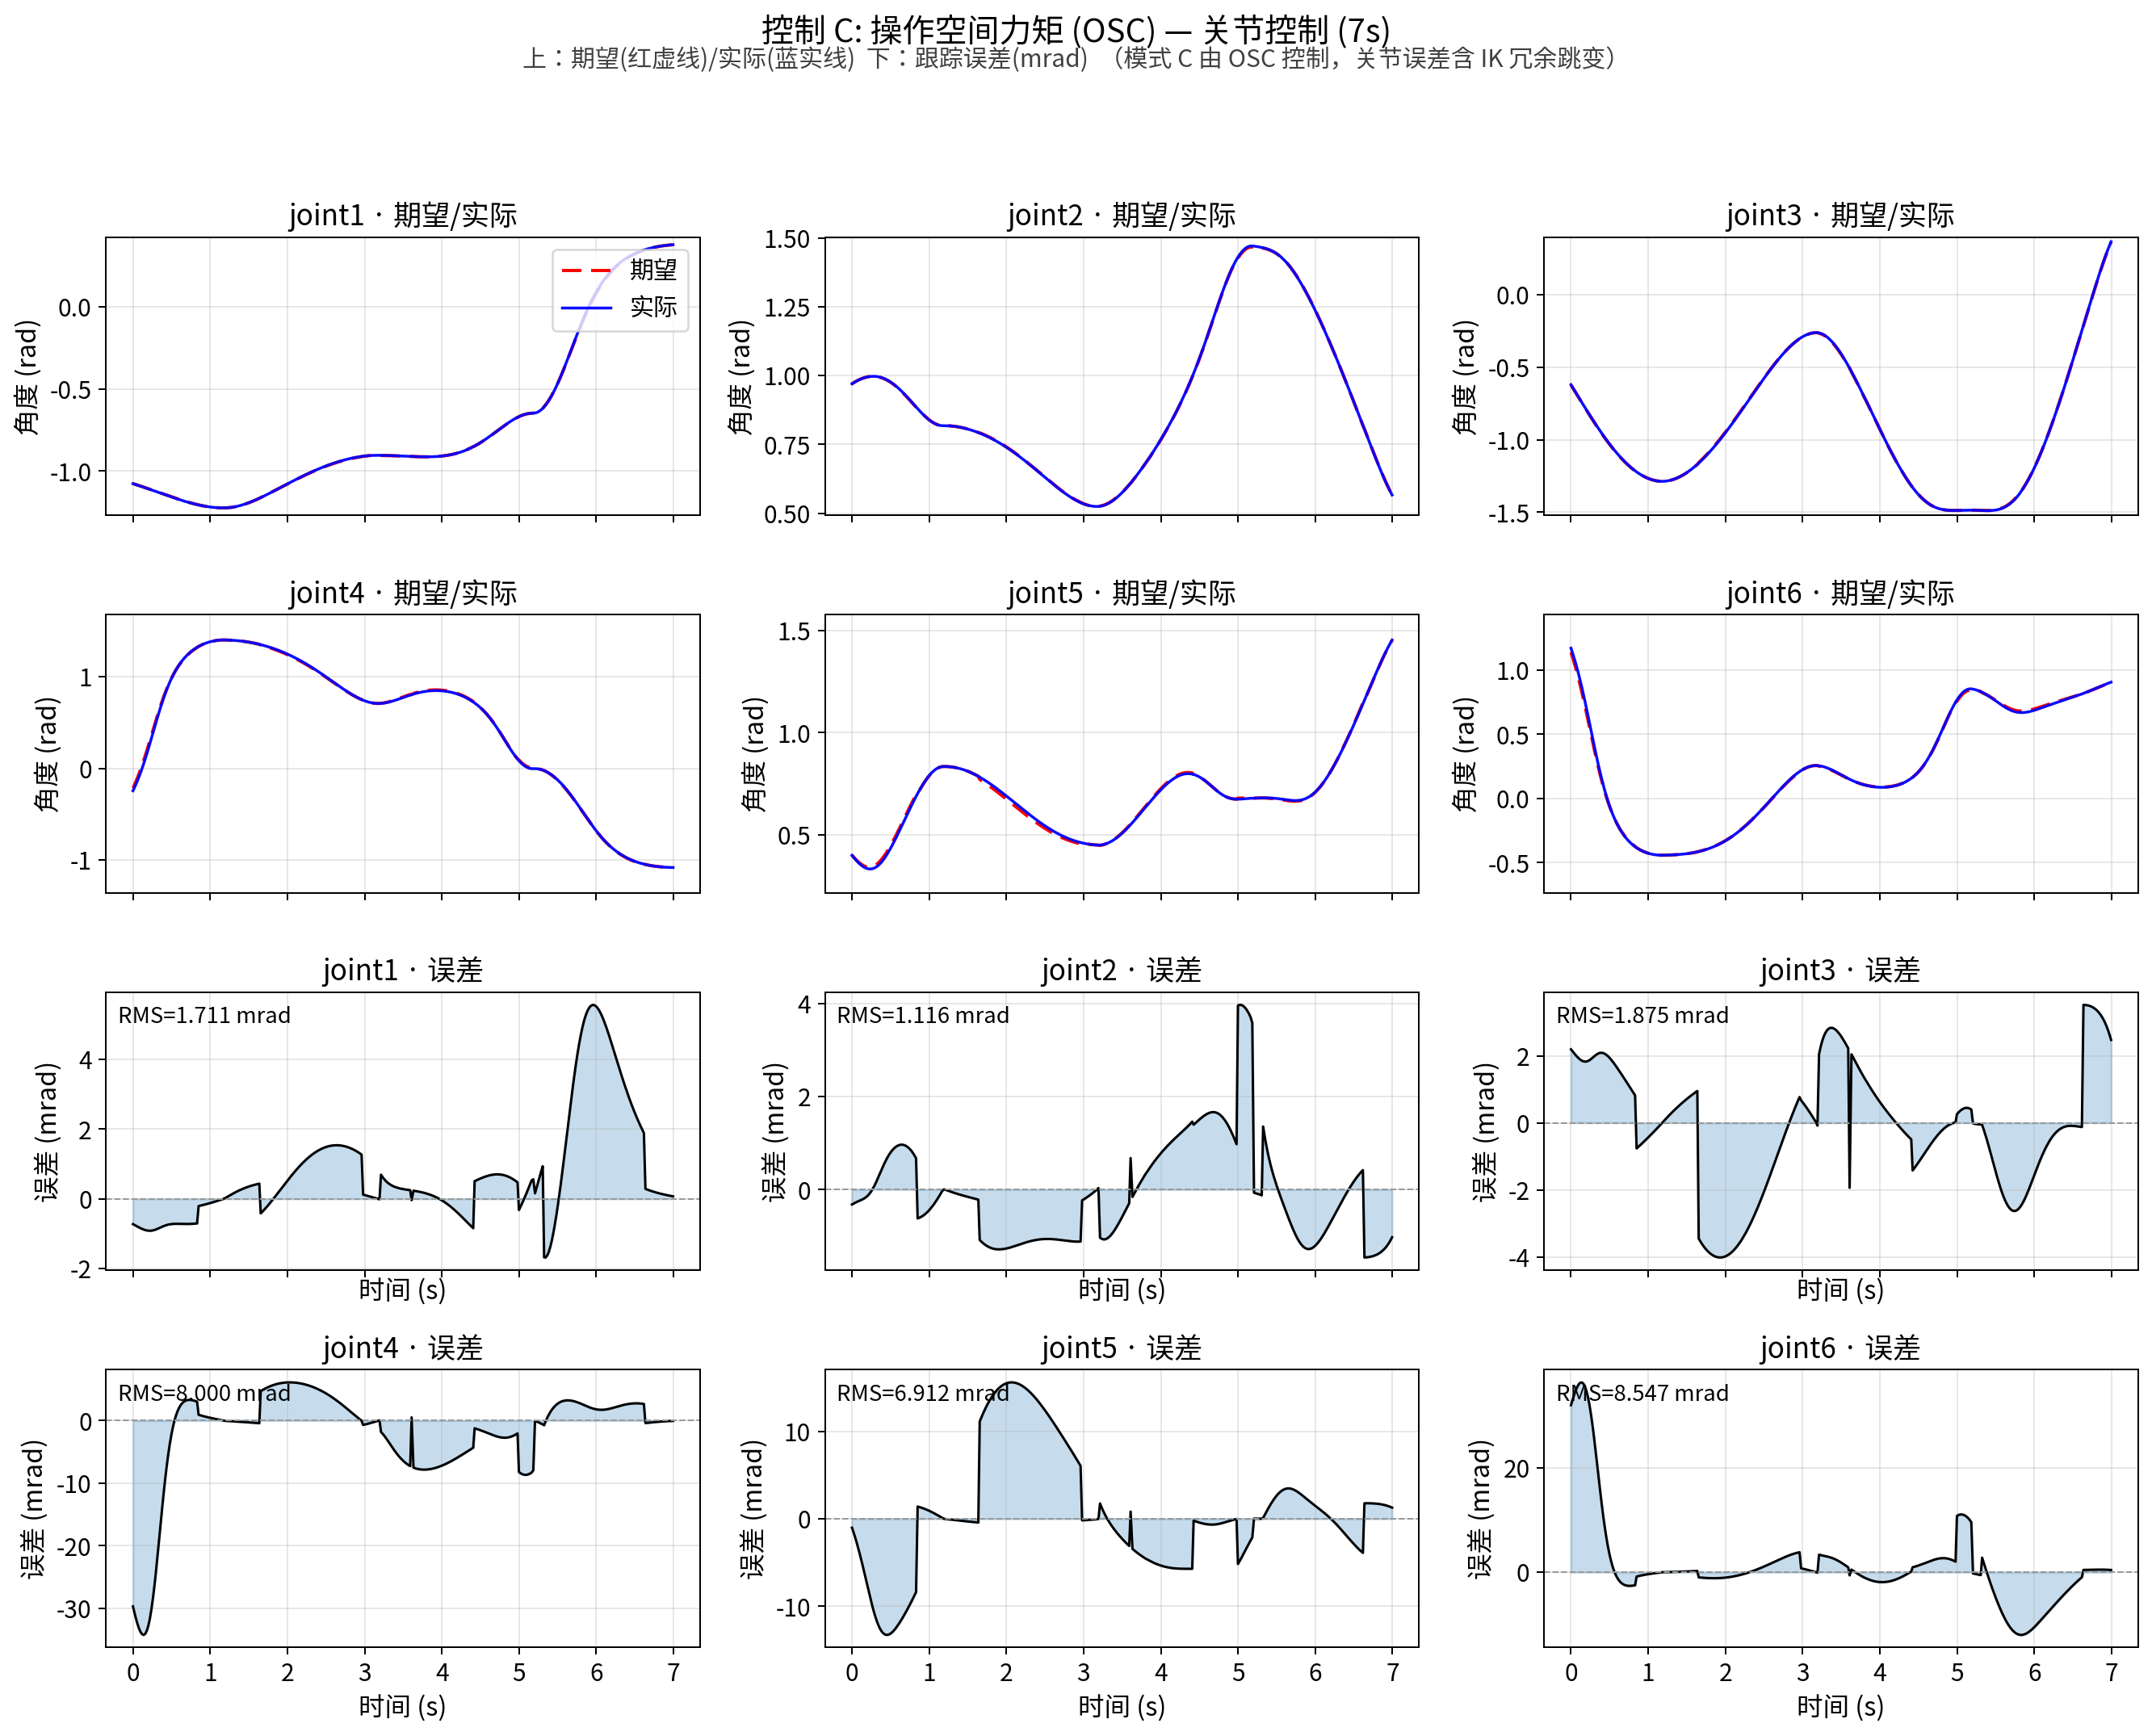
\includegraphics[width=0.92\linewidth]{mode_C_control.png}
    \caption{模式 C：IK 参考偏差 $|q-q_D|$（诊断用，非 OSC 控制目标）}
\end{figure}

\subsection{三模式综合对比}

\begin{table}[H]
  \centering
  \caption{三模式综合性能（任务空间为主）}
  \label{tab:exp-summary}
  \begin{tabular}{@{} l c c c @{}}
    \toprule
    模式 & 位置 RMS (mm) & 姿态 RMS ($^\circ$) & 关节类 RMS (rad) \\
    \midrule
    A & 0.283 & 0.037 & 0.000（参考误差） \\
    B & 2.808 & 0.258 & 0.061（跟踪误差） \\
    C & 0.363 & 0.507 & 0.014（IK 偏差，非控制目标） \\
    \bottomrule
  \end{tabular}
\end{table}

\begin{figure}[H]
    \centering
    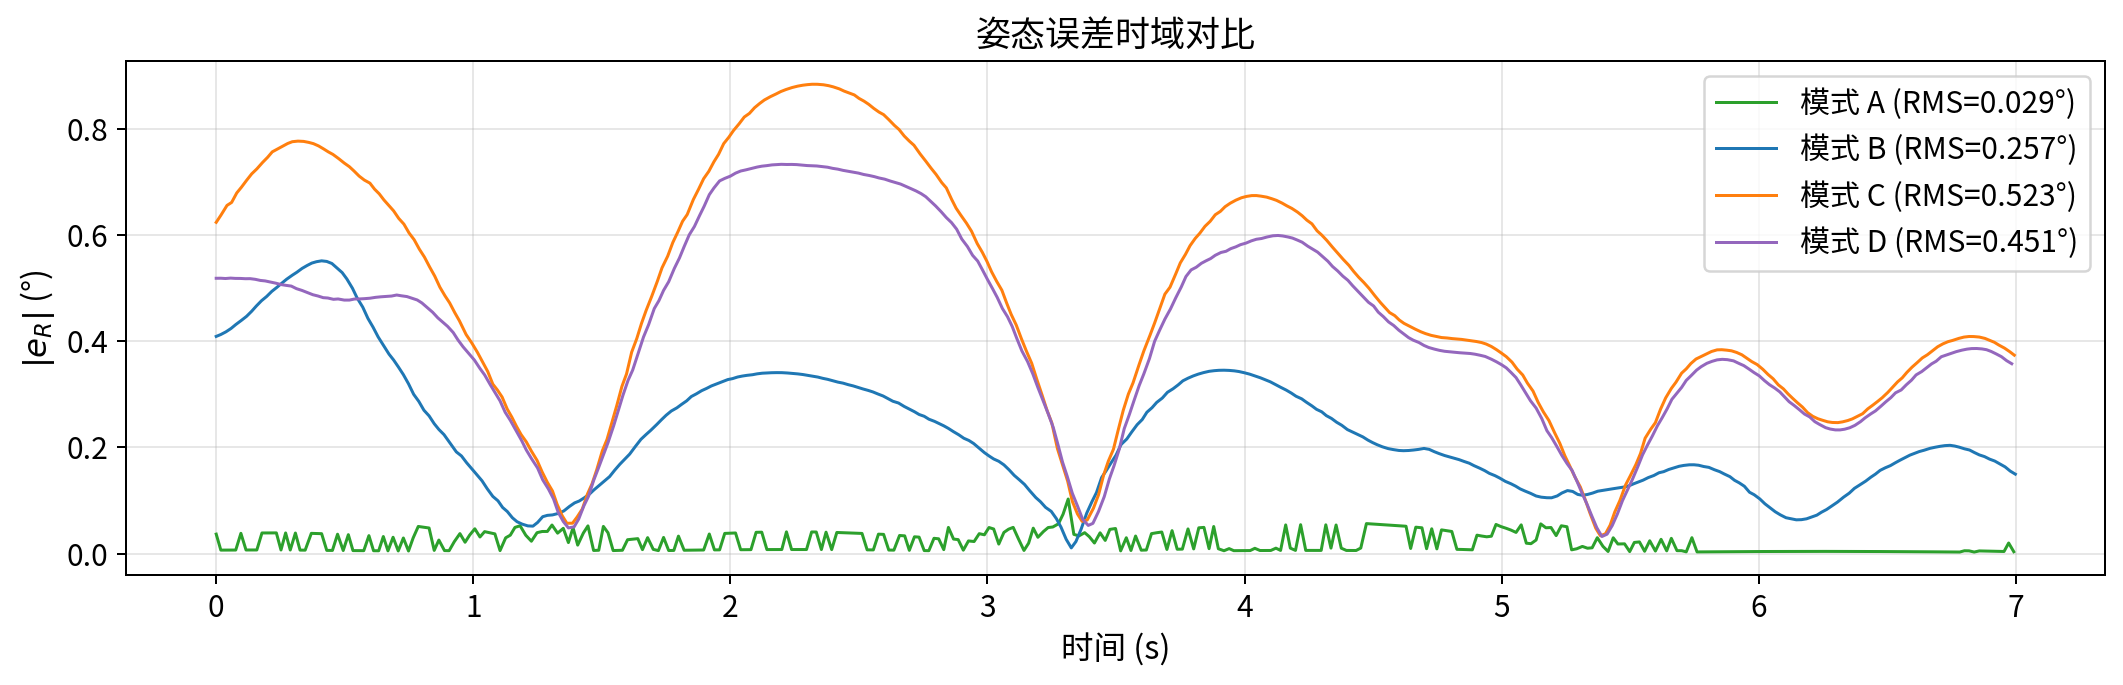
\includegraphics[width=0.92\linewidth]{mode_attitude_error.png}
    \caption{三模式姿态误差 $\|e_R\|$ 时域对比}
    \label{fig:attitude-ts}
\end{figure}
\begin{figure}[H]
    \centering
    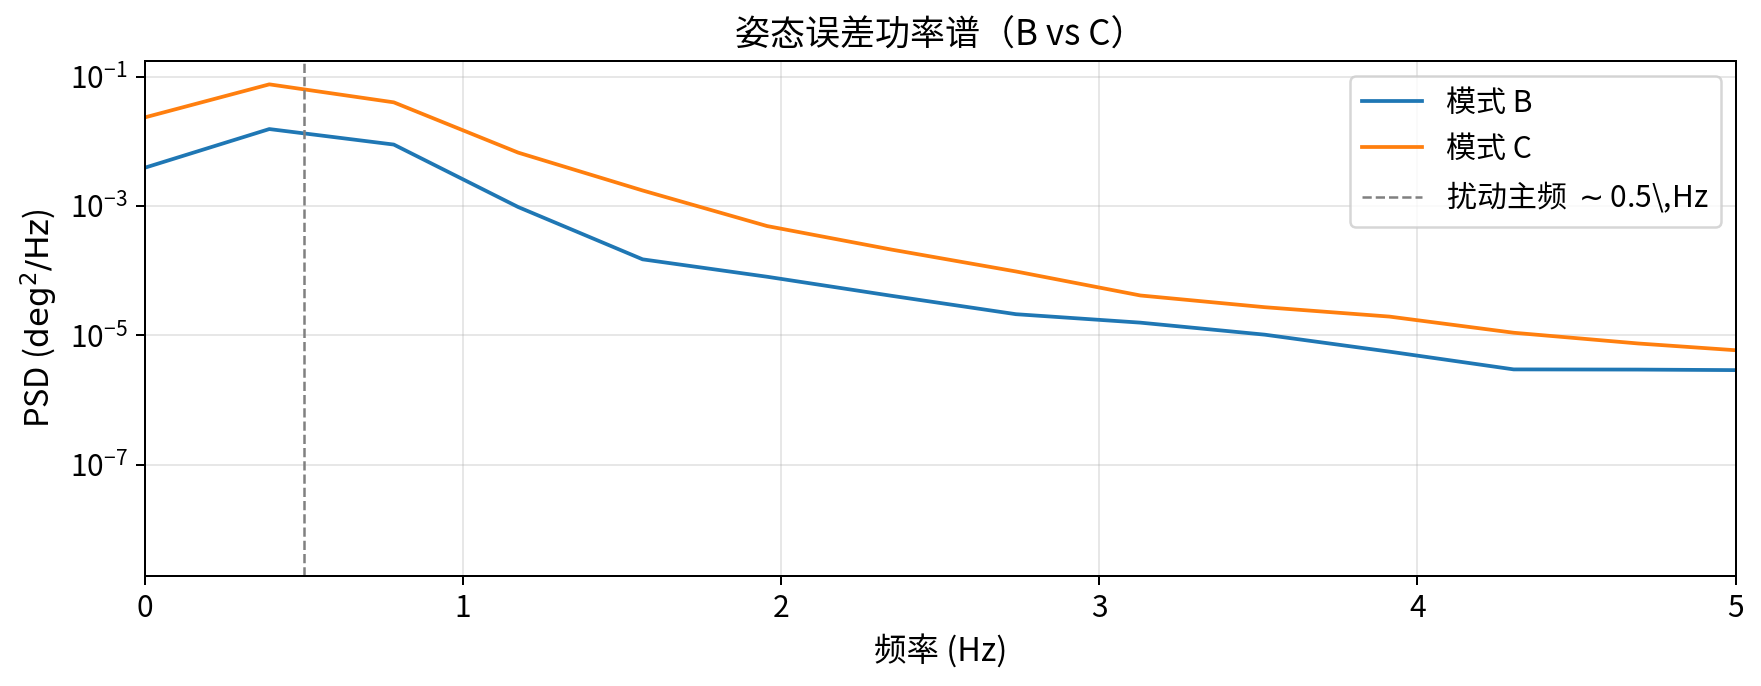
\includegraphics[width=0.85\linewidth]{mode_attitude_psd.png}
    \caption{模式 B/C 姿态误差 Welch 功率谱（扰动段内时间常数 2.0\,s，主频 $\sim$0.5\,Hz）}
    \label{fig:attitude-psd}
\end{figure}

\subsection{结果分析}
\label{sec:result-analysis}

三模式在任务空间两项主指标上的表现并不一致（表~\ref{tab:exp-summary}）：
\begin{itemize}[leftmargin=2em]
    \item \textbf{位置误差} $\|p_E-p_E^*\|$：A（0.283\,mm）$\approx$ C（0.363\,mm）$\ll$ B（2.808\,mm）；
    \item \textbf{姿态误差} $\|e_R\|$：A（0.037$^\circ$）$<$ B（0.258$^\circ$）$<$ C（0.507$^\circ$）。
\end{itemize}
因此不宜笼统表述``B 劣于 C''或``C 劣于 B''：B 在位置上远差于 C，C 在姿态上差于 B。以下分指标分析；关节类指标见~\S\ref{sec:result-joint}。

\subsubsection{位置误差：A$\approx$C}

模式 A 位置 RMS 0.283\,mm，模式 C 为 0.363\,mm，相对几何极限仅劣化
\begin{equation}
    \frac{e_{\mathrm{C}}-e_{\mathrm{A}}}{e_{\mathrm{A}}}
    = \frac{0.363-0.283}{0.283} \approx 28\%,
\end{equation}
动力学与力矩闭环引入的增量不足 30\%。同一指标下，模式 B 为 2.808\,mm，约为 A 的 9.9 倍、C 的 7.7 倍。

该对比说明：在当前扰动工况与整定参数下，位置性能的主要瓶颈在规划层（$T_B\!\rightarrow\! T_D$、$V_D$、IK），而非 OSC 动力学补偿。OSC 在引入 $M,h$、力矩限幅与 ABA 积分后，仍能将位置 RMS 维持在几何上界 0.283\,mm 的 1.3 倍以内——与 §\ref{sec:mode-a-rationale} 中``$e_{\mathrm{C}}\approx e_{\mathrm{A}}$ 表明控制层代价小''的诊断一致。后续位置精度提升应优先审计规划链路；在 $e_{\mathrm{A}}$ 未进一步压降前，单纯加大 OSC 平移增益收益有限。

\subsubsection{位置误差：B 劣于 C}
\label{sec:result-pos-bc}

本小节仅讨论位置指标 $\|p_E-p_E^*\|$：B 的 RMS 2.808\,mm、峰值 9.507\,mm（表~\ref{tab:exp-pos}），分别为 C 的 7.7 倍与 13.8 倍。根因不在``CTC 带宽不足''一句带过，而在位置通道上控制目标与误差传播路径的差异（~\S\ref{sec:control-philosophy}）。

模式 B 的位置误差经以下链路间接产生：
\begin{center}
$T_D \;\rightarrow\; \mathrm{IK} \;\rightarrow\; q_D \;\rightarrow\; \mathrm{LPF} \;\rightarrow\; \mathrm{CTC} \;\rightarrow\; q \;\rightarrow\; p_E$
\end{center}
即
\begin{equation}
    p_E \;\leftarrow\; q \;\leftarrow\; q_D \;\leftarrow\; T_D,
    \label{eq:error-chain-b}
\end{equation}
CTC 闭环最小化 $\|q-q_D\|$，实验验收的却是 $\|p_E-p_E^*\|$；二者经 $J(q)$ 与非线性正运动学耦合，无等价保证。式~\eqref{eq:error-chain-b} 在位置上的主要误差来源：
\begin{itemize}[leftmargin=2em]
    \item IK 映射误差：$q_D$ 所对应的 $p_E$ 与 $p_D$ 存在偏差；
    \item LPF 相位滞后：$\alpha=0.55$ 使 $q_D$ 滞后于 IK 输出，CTC 跟踪``过时''参考，在 0.3--1.0\,Hz 扰动频段放大 $\|p_E-p_E^*\|$；
    \item 关节跟踪误差：$\|q-q_D\|$ RMS 0.061\,rad（表~\ref{tab:exp-joint}），经 $J(q)$ 映射为末端位置偏差。
\end{itemize}

模式 C 的位置误差路径为：
\begin{center}
$T_D \;\rightarrow\; e_p \;\rightarrow\; \tau_{\mathrm{OSC}} \;\rightarrow\; p_E$
\end{center}
\begin{equation}
    p_E \;\leftarrow\; p_D \;\leftarrow\; T_D.
    \label{eq:error-chain-c}
\end{equation}
OSC 直接在任务空间最小化 $e_p=p_D-p_E$，IK 误差与 LPF 滞后不进入位置闭环。C 位置 RMS 0.363\,mm 远优于 B 的 2.808\,mm，原因在于：B 在关节空间优化 $\|q-q_D\|$，C 在任务空间优化 $\|p_E-p_E^*\|$，后者与位置验收指标一致。

图~\ref{fig:mode-B-planning} 中 B 在 2--5\,s 区间出现与 mount 扰动同步的位置误差峰（最大 9.5\,mm）；同图 C 在同一时段误差仍 $<$0.7\,mm，与上述误差链一致。

\subsubsection{姿态误差：C 劣于 B}
\label{sec:result-att-bc}

本小节仅讨论姿态指标 $\|e_R\|$：C 的 RMS 0.507$^\circ$、峰值 0.884$^\circ$（表~\ref{tab:exp-ang}），分别为 B（0.258$^\circ$、0.551$^\circ$）的 2.0 倍与 1.6 倍，亦远高于 A 的几何上界 0.037$^\circ$。这与位置维度的排序相反——C 位置优于 B，姿态却劣于 B。

该倒挂不能沿用位置误差链解释：OSC 在姿态上同样直接闭环 $e_R$，理论上与 $\|e_R\|$ 验收一致。C 姿态偏大，来自旋转通道整定与结构约束，而非``多一层 IK/LPF''。主要机理如下。

\paragraph{整定优先级（Translational priority）。}
位置 RMS 是本项目 OSC 整定的主目标（~\S9）。平移通道 $K_P=560$；旋转 $K_P=540$，数值接近，但操作空间惯量 $\Lambda$（式~\eqref{eq:lambda}）将任务加速度映射为 $\tau$ 时，平移与旋转竞争同一组关节力矩。在 6 自由度冗余臂上，满足 $e_p$ 所需 $\tau$ 往往占用力矩预算的大部分；任务加速度限幅 $\pm 220$ 进一步在平移需求大时裁剪旋转指令。结果是：位置被优先稳定，旋转通道有效带宽不足。

\paragraph{$\lambda_{\mathrm{OSC}}$ 对旋转的抑制。}
$\lambda_{\mathrm{OSC}}=0.06$ 正则化 $\Lambda^{-1}$，在 $J(q)$ 近奇异时对所有任务方向统一衰减。空中机械臂在球内扰动下频繁经过肘部奇异附近构型，旋转方向的有效增益被额外压低，而 B 的 CTC 在关节空间不受 $\Lambda$ 奇异耦合影响。

\paragraph{$\Log(SO(3))$ 线性化误差。}
姿态误差 $e_R=\Log(R_E^\top R_D)$ 仅在 $e_R$ 较小时近似线性；C 姿态峰值 0.884$^\circ$（表~\ref{tab:exp-ang}），PD 在 $\Log$ 坐标下的线性化假设减弱，等效旋转刚度随误差幅值变化。B 经 IK 将 $e_R$ 并入 $e_x$ 后映射到 $q_D$，在关节空间以近似线性方式处理，对大姿态偏差更鲁棒。

\paragraph{频域证据。}
图~\ref{fig:attitude-psd} 给出 B/C 姿态误差的 Welch 功率谱。扰动段内时间常数 2.0\,s，理论主频 $\sim$0.5\,Hz；实测 B 峰值在 0.41\,Hz，C 同频但带内（0.2--1.5\,Hz）功率为 B 的 3.5 倍。图~\ref{fig:attitude-ts} 显示 C 的 $\|e_R\|$ 在扰动频段与 mount 角运动同相起伏，而 B 幅值更低。

机理归纳：OSC 将 $V_{D,\mathrm{rot}}$ 与 $e_R$ 直接纳入任务空间闭环（式~\eqref{eq:osc}），对 mount 角速度扰动无 LPF 缓冲；在平移优先整定与 $\lambda_{\mathrm{OSC}}$ 双重约束下，0.4--0.8\,Hz 旋转误差无法被充分抑制。B 的位置虽差，但 IK+LPF 路径对 $q_D$ 的低通平滑附带衰减了部分姿态高频分量，故 $\|e_R\|$ 反而小于 C——这是关节跟踪路径在姿态维度的副效应，不改变``位置应选 C''的结论。

图~\ref{fig:rpy-rate} 给出模式 C 末端 RPY 角速度（数值差分）。扰动切换时刻角速度峰值 $>$1$^\circ$/s，与图~\ref{fig:attitude-psd} 0.4\,Hz 处 PSD 抬升对应。后续整定应在保持位置 RMS $<$0.4\,mm 前提下，对旋转 $K_P,K_D$ 与 $\lambda_{\mathrm{OSC}}$ 联合扫参，并评估任务加速度限幅对旋转通道的裁剪比例。

\begin{figure}[H]
    \centering
    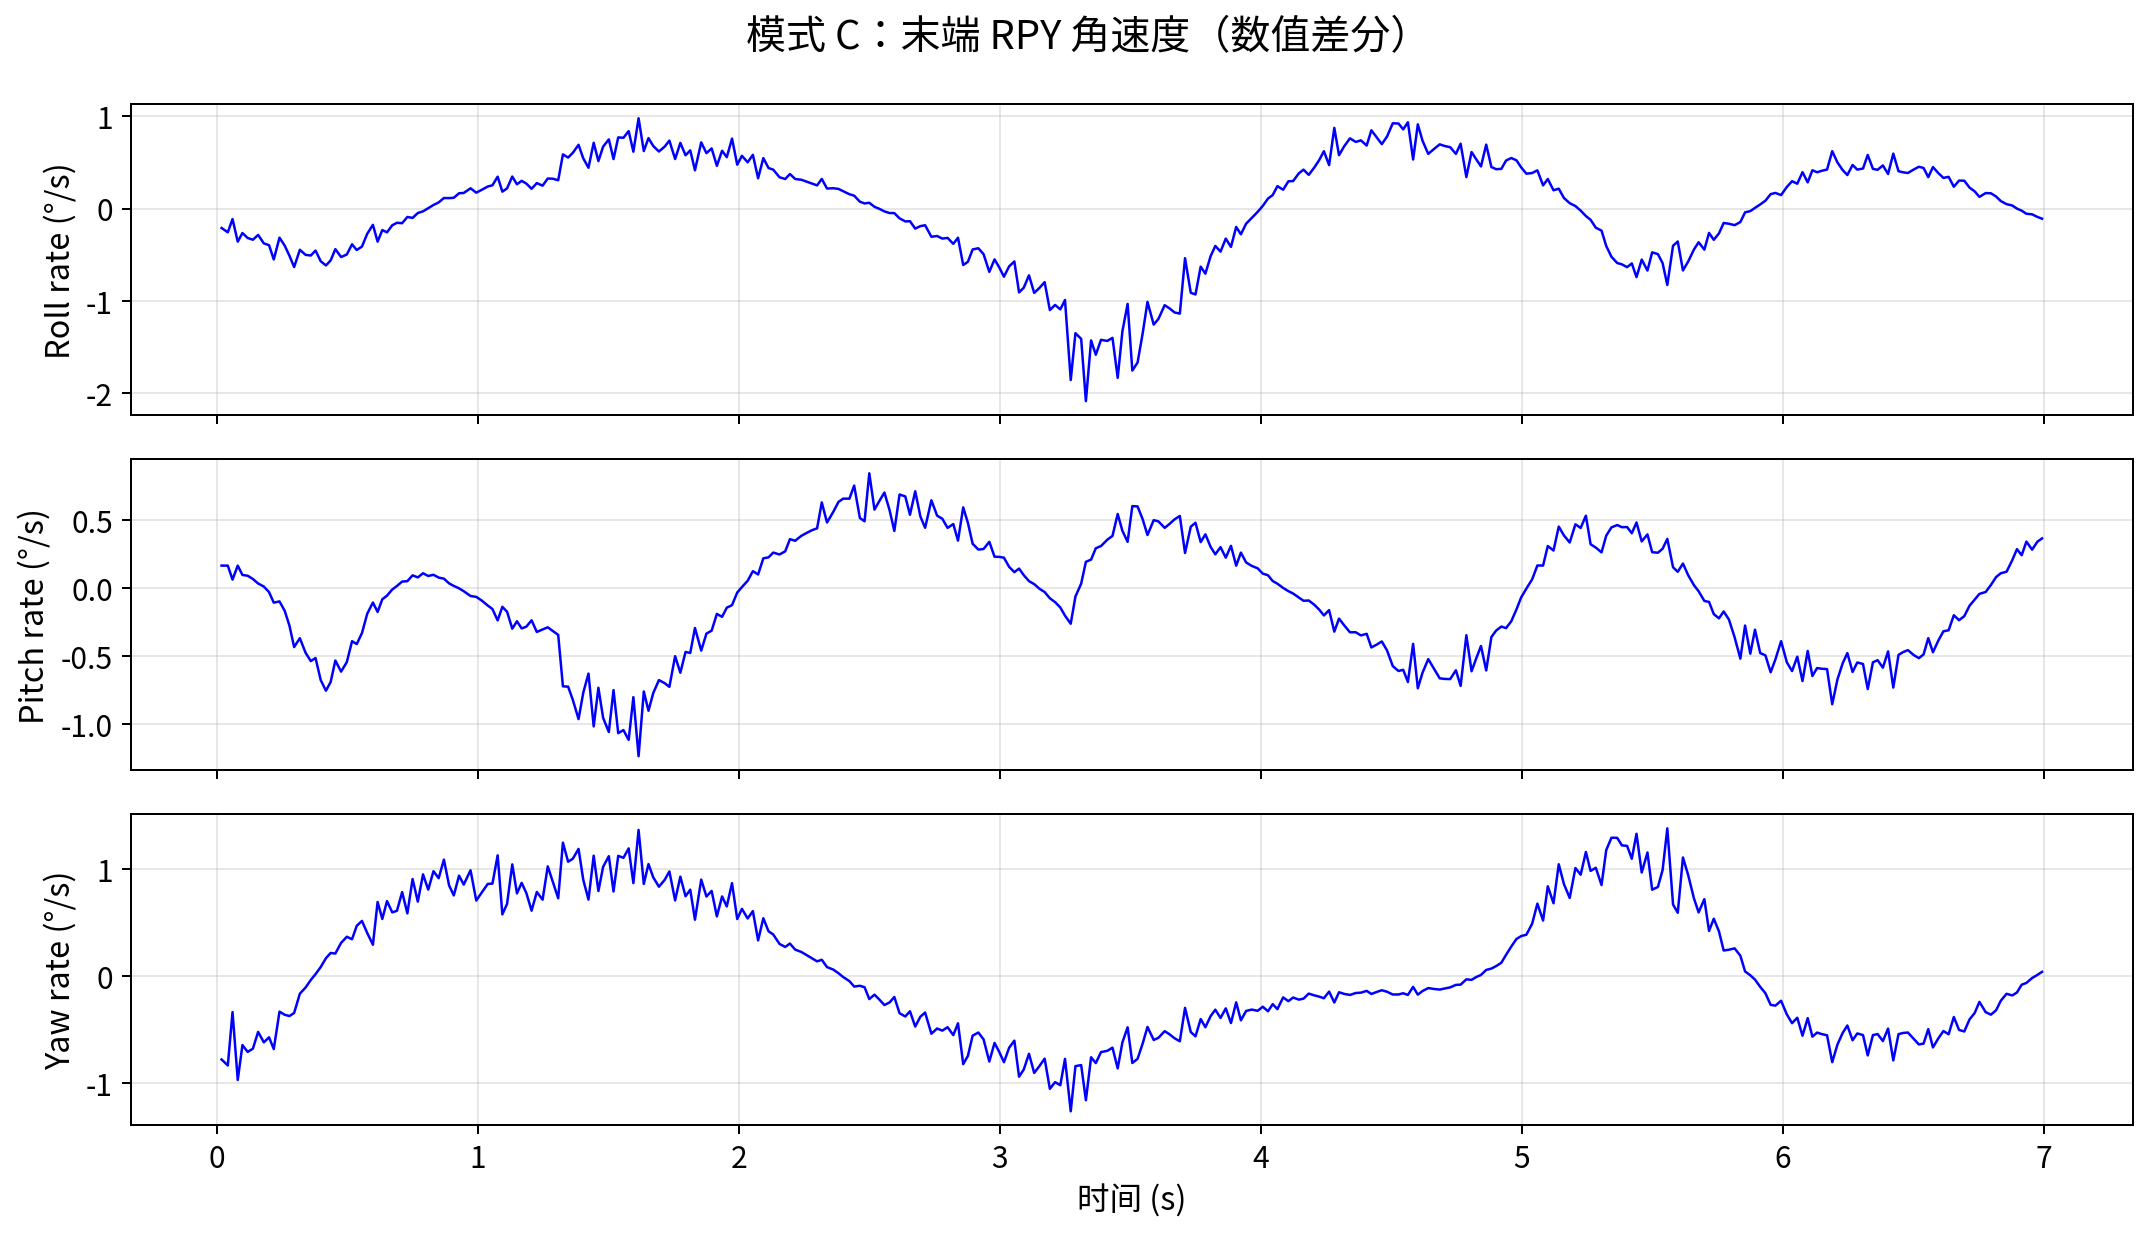
\includegraphics[width=0.92\linewidth]{mode_C_rpy_rate.png}
    \caption{模式 C：末端 RPY 角速度（数值差分）}
    \label{fig:rpy-rate}
\end{figure}

\subsubsection{模式 C 关节类指标}
\label{sec:result-joint}

C 的 $|q-q_D|$ RMS 0.014\,rad 为 IK 遥测偏差，$q_D$ 不参与 OSC 闭环；尖刺来自冗余解跳变，与姿态 RMS 无直接对应关系。C 的主评价仍为表~\ref{tab:exp-pos}、\ref{tab:exp-ang} 中的任务空间误差。

%==============================================================================
\section{参数配置与整定}
%==============================================================================

\subsection{整定说明}

\begin{itemize}[leftmargin=2em]
    \item \textbf{$\lambda_{\mathrm{IK}}=0.012$}：IK 阻尼最小二乘正则化系数；球内扰动扫参后在 500\,Hz 下迭代稳定。
    \item \textbf{$\lambda_{\mathrm{OSC}}=0.06$}：操作空间惯量正则化；统一 $V_D$ 解析方案下位置 RMS 达 0.3\,mm 量级。
    \item \textbf{$K_P,K_D$（CTC / OSC）}：对角增益，扰动工况下最小化 $\|p_E-p_E^*\|$ RMS；OSC 平移/旋转通道分别取 560/82 与 540/92。
    \item \textbf{$\alpha=0.55$（模式 B 低通）}：见 \S\ref{sec:control}；控制 IK 跳变与相位滞后的折中。
    \item \textbf{电机层 $K_P,K_D$}：MIT 阻抗（式~\eqref{eq:mit}），与 CTC/OSC 增益为不同参数组。见附录~\ref{app:params}。
\end{itemize}

完整数值见附录~\ref{app:params}。

%==============================================================================
\section{总结}
%==============================================================================

本文档规定空中机械臂末端稳定系统的分层架构、任务空间规划、三种控制模式、执行层实现与实验验证方法。真机部署主方案为 OSC；Kinematic Control 用于规划层标定。闭环仿真中，OSC 位置 RMS 0.363\,mm，CTC 2.808\,mm，Kinematic Control 几何上界 0.283\,mm。

\subsection{后续工作}

后续工作为真机验证：将当前 OSC 主方案部署至 A-L1-GAMMA 实机，接入飞控提供的 $T_B$（TF），在 MIT 阻抗执行链上闭环运行；在外场或台架扰动工况下复现仿真测试流程，检验位置/姿态 RMS 是否满足任务需求，并完善急停、通信超时与力矩限幅等安全链路。

%==============================================================================
\appendix
%==============================================================================

\section{完整参数表}
\label{app:params}

\begin{table}[H]
  \centering
  \caption{参数数值与 \texttt{yaml} 字段映射}
  \renewcommand{\arraystretch}{1.15}
  \begin{tabular}{@{} l l l @{}}
    \toprule
    符号（正文） & 数值 & \texttt{yaml} 字段（节选） \\
    \midrule
    仿真 / 真机控制频率 & 500\,Hz / 100\,Hz & \texttt{control\_rate} \\
    $z_{\mathrm{off}}$ & 0.02\,m & \texttt{mount\_base\_offset\_z} \\
    低通 $\alpha$（B） & 0.55 & \texttt{q\_des\_filter} \\
    CLIK 缩放 $\rho$（仿真 B） & 0.95 & \texttt{ctc\_vd\_scale} \\
    $\lambda_{\mathrm{IK}}$ & 0.012 & \texttt{ik} 阻尼（内嵌于求解器） \\
    $\lambda_{\mathrm{CLIK}}$ & 0.05 & \texttt{clik\_damping} \\
    $\lambda_{\mathrm{OSC}}$ & 0.06 & \texttt{osc\_lambda} \\
    OSC $K_P$ / $K_D$ & 560/82，540/92 & \texttt{kp\_task}，\texttt{kd\_task} \\
    CTC $K_P$ / $K_D$ & $[420,\ldots,320]$ / $[58,\ldots,44]$ & \texttt{joint\_kp}，\texttt{joint\_kd} \\
    CLIK $K_x$ & $[8,8,8,6,6,6]$ & \texttt{clik\_kp} \\
    仿真 $|\tau|$ 上限 & 85\,Nm & \texttt{torque\_limit} \\
    电机层 $K_P$ / $K_D$ & $[30,\ldots,1]$ / $[1,\ldots,0.1]$ & \texttt{p\_gain}，\texttt{d\_gain} \\
    真机 $|\tau|$ 上限 & 9\,Nm & \texttt{hw\_torque\_limit}，\texttt{torque\_limit} \\
    $q_{\mathrm{home}}$ & $[0,0.35,-0.55,0,0.45,0]$ & \texttt{q\_home} \\
    \bottomrule
  \end{tabular}
\end{table}

\section{ROS 2 接口}
\label{app:ros}

\begin{table}[H]
  \centering
  \caption{主要 ROS 2 话题与符号映射}
  \begin{tabular}{@{} l l l @{}}
    \toprule
    话题 & 消息类型 & 符号映射 \\
    \midrule
    \texttt{/joint\_states} & JointState & $q,\,\dot{q}$ \\
    \texttt{/stabilization\_reference} & JointState & position$\rightarrow q_D$，velocity$\rightarrow \dot{q}_D$ \\
    \texttt{/student/joint\_command} & JointState & position$\rightarrow q_D$，velocity$\rightarrow \dot{q}_D$，effort$\rightarrow \tau$ \\
    \texttt{/stabilization\_markers} & MarkerArray & 目标 $T_E^*$ 可视化 \\
    \texttt{/stabilization\_error} & Float64MultiArray & $e_x$ 分量 \\
    TF \texttt{world$\rightarrow$link6} & --- & $T_E$ \\
    \bottomrule
  \end{tabular}
\end{table}

\section{失败模式与处理}
\label{app:failure}

\begin{table}[H]
  \centering
  \caption{典型失败模式与系统响应}
  \renewcommand{\arraystretch}{1.2}
  \begin{tabular}{@{} p{3.0cm} p{4.5cm} p{6.0cm} @{}}
    \toprule
    失败模式 & 现象 & 处理策略 \\
    \midrule
    奇异位形 & $J(q)$ 近秩亏 & DLS 阻尼 $\lambda_{\mathrm{IK}},\lambda_{\mathrm{CLIK}}$；限制 $\Delta q$ 步长 \\
    IK 不收敛 & 迭代误差超阈 & 增加 refine/recovery 迭代；仍失败则沿用上一周期 $q_D$ \\
    IK 帧间跳变 & $q_D$ 尖刺 & 模式 B 低通 $\alpha=0.55$；模式 C 不跟踪 $q_D$ \\
    OSC 力矩尖峰 & $\tau$ 过大 & 任务加速度限幅 $\pm 220$；$|\tau|\le\tau_{\max}$ \\
    TF 丢失（真机） & $T_B$ 不可用 & 节流告警；\texttt{base\_source=simulated} 时回退仿真 mount \\
    NaN/Inf 指令 & 数值异常 & 执行节点拒绝写入，保持上一安全指令 \\
    通信超时 & $>$0.5\,s 无新指令 & 保持当前 $q$，$\tau$ 归零 \\
    关节近限位 & 指令超界 & 钳制 $q_D$ 至 $[q_{\min},q_{\max}]$ \\
    异步采样（测试） & 误差图伪尖刺 & 测试脚本按 stamp 配对 $q$ 与 $q_D$ \\
    \bottomrule
  \end{tabular}
\end{table}

\end{document}
